\setchapterpreamble[u]{\margintoc}
\chapter{Классические алгоритмы синтаксического анализа для строк}
\tikzsetfigurename{ClassicalParsing_}

В данной главе мы рассмотрим классические алгоритмы синтаксического анализа для строк.
Эти алгоритмы составляют фундамент, на котором далее будут построены алгоритмы поиска путей с контекстно-свободными ограничениями в графах (главы~\ref{chpt:CFPQ_CYK}--\ref{chpt:GLR}).

\section{Алгоритм CYK}
	\tikzsetfigurename{ClassicalParsing_CYK_}
\label{sec:lin_CYK}

Алгоритм CYK (Cocke-Younger-Kasami)~--- один из классических алгоритмов синтаксического анализа.
Его асимптотическая сложность в худшем случае~--- $O(n^3 \cdot |N|)$, где $n$~--- длина входной строки, а $N$~--- количество нетерминалов во входной грамматике~\sidecite{Hopcroft+Ullman/79/Introduction}.
\mytodo{Добавить псевдокод алгоритма CYK в окружении algorithm.}
\mytodo{Добавить схему доказательства корректности.}
\mytodo{При унификации примеров заменить грамматику и строку на сквозную (см.~\texttt{main.tex}).}

Для его применения необходимо, чтобы подаваемая на вход грамматика находилась в Нормальной Форме Хомского (НФХ)~\ref{sec:CNF}.
Других ограничений нет и, следовательно, данный алгоритм применим для работы с произвольными контекстно-свободными языками.
В основе алгоритма лежит принцип динамического программирования.
Используются два соображения:
\begin{enumerate}
    \item Из нетерминала $A$ выводится цепочка $\omega$ при помощи правила $A \to a$ тогда и только тогда, когда $a = \omega$:
          \[ A \derives \omega \iff \omega = a \]
    \item Из нетерминала $A$ выводится цепочка $\omega$ при помощи правила $A \to B C$ тогда и только тогда, когда существуют две цепочки $\omega_1$ и $\omega_2$ такие, что $\omega_1$ выводима из $B$, $\omega_2$ выводима из $C$ и при этом $\omega = \omega_1 \omega_2$:
          \[ A \derives[] B C \derives \omega \iff \exists \omega_1, \omega_2 : \omega = \omega_1 \omega_2, B \derives \omega_1, C \derives \omega_2 \]
          Переформулируем эти утверждения в терминах позиций в строке:
          \mytodo{Позиции в строке с 0 до $|\omega|$. Либо тут про позиции символа. Но тогда всё равно с 0 и до $|\omega|-1$}
          \[ A \derives[] B C \derives \omega \iff \exists k \in [1 \rng |\omega|] : B \derives \omega[1 \rng k], C \derives \omega[k+1 \rng |\omega|] \]
\end{enumerate}

В процессе работы алгоритма заполняется булева трехмерная матрица $M$ размера $n \times n \times  |N|$ таким образом, что
\[ M[i, j, A] = true \iff A \derives \omega[i \rng j]. \]

Первым шагом инициализируем матрицу, заполнив значения $M[i, i, A]$:
\begin{itemize}
    \item $M[i, i, A] = true$, если в грамматике есть правило $A \to \omega[i]$.\marginnote{TODO: Может надо заменить на 0 и 1?}
    \item $M[i, i, A] = false$, иначе.
\end{itemize}

Далее используем динамику: на шаге $m > 1$ предполагаем, что ячейки матрицы $M[i', j', A]$ заполнены для всех нетерминалов $A$ и пар $i', j': j' - i' < m$.
Тогда можно заполнить ячейки матрицы $M[i, j, A]$, где $j - i = m$ следующим образом:
\[ M[i, j, A] = \bigvee_{A \to B C} \bigvee_{k = i}^{j-1} M[i, k, B] \wedge M[k, j, C] \]

По итогу работы алгоритма значение в ячейке $M[0, |\omega|, S]$, где $S$~--- стартовый нетерминал грамматики, отвечает на вопрос о выводимости цепочки $\omega$ в грамматике.

\begin{example}\label{exmpl:CYK}
    \marginnote{TODO: Я бы сделал это подразделом, потому что пример всего один}
    Рассмотрим пример работы алгоритма CYK на грамматике правильных скобочных последовательностей в Нормальной Форме Хомского.
    \begin{align*}
        S   & \to A S_2 \mid \varepsilon & S_2 & \to b \mid B S_1 \mid S_1 S_3 & A & \to a \\
        S_1 & \to A S_2                  & S_3 & \to b \mid B S_1              & B & \to b
    \end{align*}

    Проверим выводимость цепочки $\omega = a a b b a b$.

    Так как трехмерные матрицы рисовать на двумерной бумаге не очень удобно, мы будем иллюстрировать работу алгоритма двумерными матрицами размера $n \times n$, где в ячейках указано множество нетерминалов, выводящих соответствующую подстроку.

    Шаг 1.
    Инициализируем матрицу элементами на главной диагонали:
    \marginnote{TODO: Я бы здесь написал снаружи нетерминалы, хотя бы в одной матричке}
    \[
        \begin{pmatrix}
            \{A\}       & \varnothing & \varnothing     & \varnothing     & \varnothing & \varnothing     \\
            \varnothing & \{A\}       & \varnothing     & \varnothing     & \varnothing & \varnothing     \\
            \varnothing & \varnothing & \{B, S_2, S_3\} & \varnothing     & \varnothing & \varnothing     \\
            \varnothing & \varnothing & \varnothing     & \{B, S_2, S_3\} & \varnothing & \varnothing     \\
            \varnothing & \varnothing & \varnothing     & \varnothing     & \{A\}       & \varnothing     \\
            \varnothing & \varnothing & \varnothing     & \varnothing     & \varnothing & \{B, S_2, S_3\}
        \end{pmatrix}
    \]

    Шаг 2.
    Заполняем диагональ, находящуюся над главной:
    \[
        \begin{pmatrix}
            \{A\}       & \varnothing & \varnothing                  & \varnothing     & \varnothing & \varnothing                  \\
            \varnothing & \{A\}       & \cellcolor{lightgray}\{S_1\} & \varnothing     & \varnothing & \varnothing                  \\
            \varnothing & \varnothing & \{B, S_2, S_3\}              & \varnothing     & \varnothing & \varnothing                  \\
            \varnothing & \varnothing & \varnothing                  & \{B, S_2, S_3\} & \varnothing & \varnothing                  \\
            \varnothing & \varnothing & \varnothing                  & \varnothing     & \{A\}       & \cellcolor{lightgray}\{S_1\} \\
            \varnothing & \varnothing & \varnothing                  & \varnothing     & \varnothing & \{B, S_2, S_3\}
        \end{pmatrix}
    \]
    В двух ячейках появились нетерминалы $S_1$ благодаря присутствию в грамматике правила $S_1 \to A S_2$.

    Шаг 3.
    Заполняем следующую диагональ:
    \[
        \begin{pmatrix}
            \{A\}       & \varnothing & \varnothing     & \varnothing                  & \varnothing & \varnothing                       \\
            \varnothing & \{A\}       & \{S_1\}         & \cellcolor{lightgray}\{S_2\} & \varnothing & \varnothing                       \\
            \varnothing & \varnothing & \{B, S_2, S_3\} & \varnothing                  & \varnothing & \varnothing                       \\
            \varnothing & \varnothing & \varnothing     & \{B, S_2, S_3\}              & \varnothing & \cellcolor{lightgray}\{S_2, S_3\} \\
            \varnothing & \varnothing & \varnothing     & \varnothing                  & \{A\}       & \{S_1\}                           \\
            \varnothing & \varnothing & \varnothing     & \varnothing                  & \varnothing & \{B, S_2, S_3\}
        \end{pmatrix}
    \]

    Шаг 4.
    И следующую за ней:
    \[
        \begin{pmatrix}
            \{A\}       & \varnothing & \varnothing     & \cellcolor{lightgray}\{S_1, S\} & \varnothing & \varnothing     \\
            \varnothing & \{A\}       & \{S_1\}         & \{S_2\}                         & \varnothing & \varnothing     \\
            \varnothing & \varnothing & \{B, S_2, S_3\} & \varnothing                     & \varnothing & \varnothing     \\
            \varnothing & \varnothing & \varnothing     & \{B, S_2, S_3\}                 & \varnothing & \{S_2, S_3\}    \\
            \varnothing & \varnothing & \varnothing     & \varnothing                     & \{A\}       & \{S_1\}         \\
            \varnothing & \varnothing & \varnothing     & \varnothing                     & \varnothing & \{B, S_2, S_3\}
        \end{pmatrix}
    \]

    Шаг 5.
    Заполняем предпоследнюю диагональ:
    \[
        \begin{pmatrix}
            \{A\}       & \varnothing & \varnothing     & \{S_1, S\}      & \varnothing & \varnothing                  \\
            \varnothing & \{A\}       & \{S_1\}         & \{S_2\}         & \varnothing & \cellcolor{lightgray}\{S_2\} \\
            \varnothing & \varnothing & \{B, S_2, S_3\} & \varnothing     & \varnothing & \varnothing                  \\
            \varnothing & \varnothing & \varnothing     & \{B, S_2, S_3\} & \varnothing & \{S_2, S_3\}                 \\
            \varnothing & \varnothing & \varnothing     & \varnothing     & \{A\}       & \{S_1\}                      \\
            \varnothing & \varnothing & \varnothing     & \varnothing     & \varnothing & \{B, S_2, S_3\}
        \end{pmatrix}
    \]

    Шаг 6.
    Завершаем выполнение алгоритма:
    \marginnote{TODO: Надо подумать как сделать так, чтобы не вылезало}
    \[
        \begin{pmatrix}
            \{A\}       & \varnothing & \varnothing     & \{S_1, S\}      & \varnothing & \cellcolor{lightgray}\{S_1, S\} \\
            \varnothing & \{A\}       & \{S_1\}         & \{S_2\}         & \varnothing & \{S_2\}                         \\
            \varnothing & \varnothing & \{B, S_2, S_3\} & \varnothing     & \varnothing & \varnothing                     \\
            \varnothing & \varnothing & \varnothing     & \{B, S_2, S_3\} & \varnothing & \{S_2, S_3\}                    \\
            \varnothing & \varnothing & \varnothing     & \varnothing     & \{A\}       & \{S_1\}                         \\
            \varnothing & \varnothing & \varnothing     & \varnothing     & \varnothing & \{B, S_2, S_3\}
        \end{pmatrix}
    \]

    Стартовый нетерминал находится в верхней правой ячейке, а значит цепочка $a a b b a b$ выводима в нашей грамматике.
\end{example}

\begin{example}
    Теперь выполним алгоритм на цепочке $\omega=abaa$.

    Шаг 1.
    Инициализируем таблицу:
    \[
        \begin{pmatrix}
            \{A\}       & \varnothing     & \varnothing & \varnothing \\
            \varnothing & \{B, S_2, S_3\} & \varnothing & \varnothing \\
            \varnothing & \varnothing     & \{A\}       & \varnothing \\
            \varnothing & \varnothing     & \varnothing & \{A\}
        \end{pmatrix}
    \]

    Шаг 2.
    Заполняем следующую диагональ:
    \[
        \begin{pmatrix}
            \{A\}       & \cellcolor{lightgray}\{S_1, S\} & \varnothing & \varnothing \\
            \varnothing & \{B, S_2, S_3\}                 & \varnothing & \varnothing \\
            \varnothing & \varnothing                     & \{A\}       & \varnothing \\
            \varnothing & \varnothing                     & \varnothing & \{A\}
        \end{pmatrix}
    \]

    Больше ни одну ячейку в таблице заполнить нельзя и при этом стартовый нетерминал отсутствует в правой верхней ячейке, а значит эта строка не выводится в грамматике правильных скобочных последовательностей.
\end{example}

Рассмотренный выше вариант алгоритма решает только задачу выводимости: в ячейках матрицы хранятся множества нетерминалов, а информация, необходимая для восстановления леса разбора, отбрасывается.
Модифицируем алгоритм так, чтобы по завершении работы можно было восстановить сжатое представление леса разбора (SPPF, раздел~\ref{sec:SPPF}) в варианте Рекерса (определение~\ref{def:basicSPPF}).

Основная идея состоит в том, чтобы хранить в ячейке матрицы не просто множество нетерминалов, а множество троек вида $(A, k, p)$, где $A$~--- нетерминал, $k$~--- точка расщепления, а $p$~--- номер продукции грамматики, приведённой к НФХ.
Клетка $M[i,j]$ матрицы, где $0 \leq i \leq j \leq n-1$, соответствует подстроке $w[i..j]$, то есть символам с индексами от $i$ до $j$ включительно.
Тройка $(A, k, p)$ в клетке $M[i,j]$ означает, что нетерминал $A$ выводит подстроку $w[i..j]$ при помощи продукции с номером $p$.
Для бинарной продукции $A \to B C$ точка расщепления $k$ ($i \leq k < j$) задаёт разбиение подстроки: $B$ выводит $w[i..k]$, а $C$ выводит $w[k+1..j]$.
Для терминальной продукции $A \to a$ точка расщепления не используется, и на её месте хранится индекс символа, то есть $k = i$.

Инициализация выполняется так же, как в исходном алгоритме: для каждой терминальной продукции $A \to a$ с номером $p$ и каждого индекса $i \in [0 \rng n-1]$ такого, что $w[i] = a$, в клетку $M[i,i]$ добавляется тройка $(A, i, p)$.

Динамика также повторяет исходный алгоритм, но фиксирует точку расщепления и номер продукции: для каждой бинарной продукции $A \to B C$ с номером $p$ и каждой точки расщепления $k$, $i \leq k < j$, если в клетке $M[i,k]$ найдётся тройка с нетерминалом $B$, а в клетке $M[k+1,j]$~--- тройка с нетерминалом $C$, то в клетку $M[i,j]$ добавляется тройка $(A, k, p)$.

По завершении основного прохода, если стартовый нетерминал $S$ присутствует в правой верхней клетке $M[0,n-1]$, то вывод успешен и SPPF восстанавливается рекурсивным проходом от корня.
В SPPF вершины нумеруются позициями между символами (определение~\ref{def:PositionInString}): клетке $M[i,j]$ соответствует символьная вершина $X_{i,j+1}$, а точке расщепления $k$~--- позиция $k+1$.
Для каждой тройки $(A, k, p)$ из клетки $M[i,j]$:
\begin{itemize}
    \item создаём (или переиспользуем уже созданную) символьную вершину $X_{i,j+1}$;
    \item создаём вершину-продукцию с номером $p$ и соединяем её с символьной вершиной $X_{i,j+1}$;
    \item если $p$~--- терминальная продукция $A \to a$, то создаём терминальный лист $a_{i,i+1}$ и соединяем с ним вершину-продукцию;
    \item если $p$~--- бинарная продукция $A \to B C$, то рекурсивно обрабатываем клетки $M[i,k]$ (для $B$) и $M[k+1,j]$ (для $C$), после чего соединяем вершину-продукцию с символьными вершинами $X_{i,k+1}$ и $X_{k+1,j+1}$.
\end{itemize}
Переиспользование символьных вершин по паре $(A, i, j)$ даёт разделение общих поддеревьев, а переиспользование вершин-продукций~--- упаковку альтернатив (см.~определение~\ref{def:basicSPPF}).
Заметим, что в матрице могут присутствовать тройки, не достигаемые при проходе от корня; в SPPF они не попадают.

\begin{example}\label{exmpl:CYK_SPPF}
    Проиллюстрируем работу модифицированного алгоритма на неоднозначной грамматике
    \begin{alignat*}{3}
    1) \ & S &&\rightarrow a \\
    2) \ & S &&\rightarrow S\ S \\
    3) \ & S &&\rightarrow S\ S\ S \\
    \end{alignat*}
    и цепочке $w = a a a$.
    Приведём грамматику к НФХ (раздел~\ref{sec:CNF}): продукцию $S \to S S S$ длины три заменим на две бинарные продукции, введя новый нетерминал $N_1$:
    \begin{alignat*}{3}
    1) \ & S &&\rightarrow a \\
    2) \ & S &&\rightarrow S\ S \\
    3) \ & S &&\rightarrow S\ N_1 \\
    4) \ & N_1 &&\rightarrow S\ S \\
    \end{alignat*}

    Длина цепочки равна $3$, поэтому заполняются клетки $M[i,j]$ для $0 \leq i \leq j \leq 2$; строка входа имеет вид
    \[
    \begin{pNiceMatrix}[margin=2pt] a & a & a \end{pNiceMatrix}
    \]

    Шаг 1.
    Для каждого индекса $i$ добавляем в клетку $M[i,i]$ тройку, отвечающую продукции $1)$ $S \to a$:
    \[
    \begin{pNiceMatrix}[color-inside,first-row,code-for-first-row = \arabic{jCol},first-col,code-for-first-col = \arabic{iRow}]
     &  &  &  \\
     & \cellcolor{yellow}{\{(S, 0, 1)\}} & \cdot & \cdot \\
     & \cdot & \cellcolor{yellow}{\{(S, 1, 1)\}} & \cdot \\
     & \cdot & \cdot & \cellcolor{yellow}{\{(S, 2, 1)\}} \\
    \end{pNiceMatrix}
    \]

    Шаг 2.
    Заполняем клетки, соответствующие подстрокам длины $2$.
    Для клетки $M[0,1]$ единственная точка расщепления~--- $k = 0$; так как и $M[0,0]$, и $M[1,1]$ содержат нетерминал $S$, по продукции $2)$ $S \to S S$ получаем тройку $(S, 0, 2)$, а по продукции $4)$ $N_1 \to S S$~--- тройку $(N_1, 0, 4)$.
    Аналогично для клетки $M[1,2]$ с точкой расщепления $k = 1$ получаем тройки $(S, 1, 2)$ и $(N_1, 1, 4)$:
    \[
    \begin{pNiceMatrix}[color-inside,first-row,code-for-first-row = \arabic{jCol},first-col,code-for-first-col = \arabic{iRow}]
     &  &  &  \\
     & \{(S, 0, 1)\} & \cellcolor{yellow}{\{(N_1, 0, 4), (S, 0, 2)\}} & \cdot \\
     & \cdot & \{(S, 1, 1)\} & \cellcolor{yellow}{\{(N_1, 1, 4), (S, 1, 2)\}} \\
     & \cdot & \cdot & \{(S, 2, 1)\} \\
    \end{pNiceMatrix}
    \]

    Шаг 3.
    Заполняем клетку $M[0,2]$, соответствующую всей цепочке.
    Для точки расщепления $k = 0$ используются клетки $M[0,0]$ и $M[1,2]$: по продукции $2)$ получаем тройку $(S, 0, 2)$, по продукции $3)$ $S \to S N_1$~--- тройку $(S, 0, 3)$, а по продукции $4)$~--- тройку $(N_1, 0, 4)$.
    Для точки расщепления $k = 1$ используются клетки $M[0,1]$ и $M[2,2]$: по продукции $2)$ получаем тройку $(S, 1, 2)$, а по продукции $4)$~--- тройку $(N_1, 1, 4)$:
    \begin{center}
    \resizebox{\textwidth}{!}{$\begin{pNiceMatrix}[color-inside,first-row,code-for-first-row = \arabic{jCol},first-col,code-for-first-col = \arabic{iRow}]
     &  &  &  \\
     & \{(S, 0, 1)\} & \{(N_1, 0, 4), (S, 0, 2)\} & \cellcolor{yellow}{\{(N_1, 0, 4), (N_1, 1, 4), (S, 0, 2), (S, 0, 3), (S, 1, 2)\}} \\
     & \cdot & \{(S, 1, 1)\} & \{(N_1, 1, 4), (S, 1, 2)\} \\
     & \cdot & \cdot & \{(S, 2, 1)\} \\
    \end{pNiceMatrix}$}
    \end{center}

    Стартовый нетерминал $S$ присутствует в правой верхней клетке $M[0,2]$, причём тремя различными способами, поэтому цепочка $a a a$ выводима.
    Восстановим SPPF проходом от корня (рис.~\ref{fig:sppf_cyk}).
    В нём символьные вершины помечены символом и диапазоном позиций (например, $S [0,3]$), а вершины-продукции~--- парой <<точка расщепления, номер продукции>>.
    У корня $S [0,3]$ три вершины-продукции~--- $(1,2)$, $(1,3)$ и $(2,2)$~--- по одной на каждый из трёх способов вывести всю цепочку.
    Обратим внимание на две особенности.
    Во-первых, символьные вершины $S [0,1]$, $S [1,2]$ и $S [2,3]$ переиспользуются: каждая из них имеет по три родительские вершины-продукции, что отражает неоднозначность грамматики~--- три дерева вывода цепочки $a a a$ <<упаковываются>> в один SPPF.
    Во-вторых, в клетке $M[0,2]$ присутствуют также тройки $(N_1, 0, 4)$ и $(N_1, 1, 4)$, однако соответствующая им символьная вершина $N_1 [0,3]$ недостижима из корня (стартовый нетерминал $S$ не обращается к $N_1$, покрывающему всю цепочку), поэтому в SPPF она не попадает.

    \begin{figure}
        \begin{center}
            \resizebox{0.8\textwidth}{!}{\begin{tikzpicture}
  \graph [layered layout, nodes={draw}, grow'=down, level sep=1.5cm, sibling sep=1.0cm] {
    n0 [as={S [0,3]}, fill=green!30];
    n1 [as={1, 2}];
    n2 [as={S [0,1]}];
    n3 [as={0, 1}];
    n4 [as={a\_\{0,1\}}];
    n5 [as={S [1,3]}];
    n6 [as={2, 2}];
    n7 [as={S [1,2]}];
    n8 [as={1, 1}];
    n9 [as={a\_\{1,2\}}];
    n10 [as={S [2,3]}];
    n11 [as={2, 1}];
    n12 [as={a\_\{2,3\}}];
    n13 [as={1, 3}];
    n14 [as={N\_1 [1,3]}];
    n15 [as={2, 4}];
    n16 [as={2, 2}];
    n17 [as={S [0,2]}];
    n18 [as={1, 2}];
    n0 -> n1;
    n0 -> n13;
    n0 -> n16;
    n1 -> n2;
    n1 -> n5;
    n2 -> n3;
    n3 -> n4;
    n5 -> n6;
    n6 -> n7;
    n6 -> n10;
    n7 -> n8;
    n8 -> n9;
    n10 -> n11;
    n11 -> n12;
    n13 -> n2;
    n13 -> n14;
    n14 -> n15;
    n15 -> n7;
    n15 -> n10;
    n16 -> n10;
    n16 -> n17;
    n17 -> n18;
    n18 -> n2;
    n18 -> n7;
  };
\end{tikzpicture}
}
        \end{center}
        \caption{SPPF для цепочки $a a a$ в неоднозначной грамматике $S \to a \mid S S \mid S S S$, построенный версией алгоритма CYK с сохранением троек.}
        \label{fig:sppf_cyk}
    \end{figure}
\end{example}

\section{Алгоритм Валианта}

Алгоритм Валианта~\sidecite{Valiant:1975:GCR:1739932.1740048} сводит задачу синтаксического анализа линейного входа к задаче перемножения булевых матриц, что позволяет достичь субкубической сложности $O(n^\omega)$ для произвольных КС-грамматик, где $\omega$~--- экспонента матричного умножения.
В отличие от CYK, алгоритм Валианта использует возведение матриц в квадрат (repeated squaring) вместо троекратного вложенного цикла.
Однако этот подход существенно опирается на возможность упорядочить обход матрицы, что не обобщается на случай произвольных графов~\sidecite{Yannakakis}.

\section{Построение множеств first и follow}

\section{Нисходящий синтаксический анализ}
\label{sec:TopDown}
\tikzsetfigurename{TopDown_}

\subsection{Рекурсивный спуск}

Идея рекурсивного спуска основана на использовании программного стека вызовов в качестве стека магазинного автомата. Достигается это следующим образом.
\begin{itemize}
  \item Для каждого нетерминала создаётся функция, принимающая ещё не обработанный остаток строки и возвращающая пару: результат вывода префикса данной строки из соответствующего нетерминала и не обработанный остаток строки. В случае распознавателя результат вывода~--- логическое значение (выводится/не выводится).
  \item Каждая такая функция реализовывает обработку цепочки согласно правым частям правил для соответствующих нетерминалов: считывание символа входа при обработке терминального символа, вызов соответствующей функции при обработке нетерминального.
\end{itemize}

У такого подхода есть два ограничения:
\begin{enumerate}
  \item Не работает с леворекурсивными грамматиками, то есть грамматиками, вывод в которых может принимать следующий вид:
  \[
  S \to \cdots \to \underline{N_i} \alpha \to \cdots \underline{N_i} \beta \to \cdots \omega
  \]
  \item Шаги должны быть однозначными.
\end{enumerate}

\begin{example}

Построим функцию рекурсивного спуска для продукции $S \rightarrow aSbS \mid \varepsilon$.

\begin{algorithm}
  \floatname{algorithm}{Listing}
%\begin{algorithmic}[1]
%\caption{Функция рекурсивного спуска}
%\Function{S}{$\omega$}
%    \If {(len$(\omega)=0$)}
%    \Comment{{\footnotesize Пустая цепочка выводима из $S$}}
%    \State{\Return \textit{(true, $\omega$)}}
%    \EndIf

%    \If{$(\omega = a :: tl)$}
%        \Comment{{\footnotesize Выводимая из $S$ подстрока должна начинаться с $a$}}
%        \State{$res,tl' = $ S($tl$)}
%        \Comment{{\footnotesize Затем должна идти подстрока, выводимая из $S$}}
%        \If{res \&\&  $tl' = b :: tl''$}
%           \Comment{{\footnotesize Если вызов закончился успешно, то надо проверить, что следующий символ --- это $b$}}
%           \State{\Return $S(tl'')$}
%           \Comment{{\footnotesize И снова попробовать вывести префикс из $S$}}
%         \Else
%           \State{\Return \textit{(false, $tl'$)}}
%        \EndIf
%    \Else
%        \State{\Return \textit{(false, $\omega$)}}
%    \EndIf
%\EndFunction

%\end{algorithmic}
\end{algorithm}
\end{example}

Если возвращаемое значение этой функции~--- пара вида \textit{(true, [])}, то разбор завершился успехом.

Данный подход применяется как для ручного написания синтаксических нализаторов, так и при генерации анализаторов по грамматике.

\subsection{LL(k)-алгоритм синтаксического анализа}

LL(k)~--- алгоритм синтаксического анализа~--- нисходящий анализ без отката, но с предпросмотром.
Решение о том, какую продукцию применять, принимается на основании k следующих за текущим символом.
Временная сложность алгоритма $O(n)$, где $n$~--- длина слова.

Алгоритм использует входной буфер, стек для хранения промежуточных данных и таблицу анализатора, которая управляет процессом разбора.
В ячейке таблицы указано правило, которое нужно применять, если рассматривается нетерминал $A$, а следующие $m$ символов строки~--- $t_{1} \dots t_{m}$, где $m \leq k$.
Также в таблице выделена отдельная колонка для $\$$~--- маркера конца строки.

\begin{center}
  \begin{tabular}{ c || c | c | c | c }
             & $\dots$ & $t_{1} \dots t_{m}$ & $\dots$ & $\$$ \\ \hline
    $\dots$  & $\dots$ & $\dots$ & $\dots$ & $\dots$ \\ \hline
    $A$  & $\dots$ & $A \to \alpha$ & $\dots$ & $\dots$ \\ \hline
    $\dots$  & $\dots$ & $\dots$ & $\dots$ & $\dots$
  \end{tabular}
\end{center}

Для построения таблицы вычисляются множества $\first[k]$ и $\follow[k]$, определение и алгоритмы вычисления которых подробно разобраны в разделе~\ref{sec:FirstAndFollow}.
Пример вычисления для конкретной грамматики приведён в примере~\ref{exmpl:first_follow}.

Управляющая таблица LL(k) анализатора заполняется следующим образом: продукции $A \to \alpha, \alpha \neq \varepsilon$ помещаются в ячейки $(A, a)$, где $a \in \first(\alpha)$, продукции $A \to \alpha$~--- в ячейки $(A, a)$, где $a \in \follow(A)$, если $\varepsilon \in \first(\alpha)$

\begin{example}

Пример таблицы для грамматики $S \to aSbS \mid \varepsilon$

\begin{center}
\begin{tabular}{ r || c | c || c | c | c }
N & $\first$ & $\follow$ & a & b & $\$ $ \\ \hline
$S$ & $\{ a, \varepsilon \}$ & $\{ b, \$ \}$ & $S \rightarrow aSbS$ & $S \rightarrow \varepsilon$ & $S \rightarrow \varepsilon$
\end{tabular}
\end{center}

\end{example}

Однако, не для всех грамматик по множествам $\first[k]$ и $\follow[k]$ возможно выбрать применяемую продукцию, а значит, нельзя однозначно построить таблицу, необходимую для работы алгоритма, поэтому данный алгоритм применим только для грамматик особого класса~--- LL(k).

\begin{definition}
  LL(k) грамматика~--- грамматика, для которой на основании множеств $\first[k]$ и $\follow[k]$ можно однозначно определить, какую продукцию применять.
\end{definition}

Важно заметить, что при больших $k$ управляющая таблица сильно разрастается, поэтому на практике данный алгоритм применим для небольших значений $k$.

Интерпретатор автомата принимает входную строку и построенную управляющую таблицу и работает следующим образом.
В каждый момент времени конфигурация автомата это позиция во входной строке и стек.
В начальный момент времени стек пуст, а позиция во входной строке соответствует её началу.
На первом шаге в стек добавляются последовательно сперва символ конца строки, затем стартовый нетерминал.
На каждом шаге анализируется существующая конфигурация и совершается одно из действий.
\begin{itemize}
\item Если текущая позиция~--- конец строки и вершина стека~--- символ конца строки, то успешно завершаем разбор.
\item Если текущая вершина стека~--- терминал, то проверяем, что позиция в строке соответствует этому терминалу. Если да, то снимаем элемент со стека, сдвигаем позицию на единицу и продолжаем разбор. Иначе завершаем разбор с ошибкой.
\item Если текущая вершина стека~--- нетерминал $N_i$ и текущий входной символ $t_j$, то ищем в управляющей таблице ячейку с координатами $(N_i, t_j)$ и записываем на стек содержимое этой ячейки.
\end{itemize}

\begin{example}Пример работы LL анализатора.
Рассмотрим грамматику $S \to aSbS \mid \varepsilon$ и выводимое слово $\omega = abab$.

Рассмотрим пошагово работу алгоритма c построением дерева, будем использовать таблицу, построенную в предыдущем примере:

\begin{enumerate}
  \item Начало работы.

  Стек: \,
    \begin{tabular}[c]{ |c| }
        \\ \hline
        \$ \\ \hline
    \end{tabular}
    \qquad  \qquad \qquad  \qquad входное слово: \,
    \begin{tabular}[c]{ |c|c|c|c|c| }
        \hline
        \textcolor{red}{a} & b & a & b & \$ \\ \hline
    \end{tabular}

Финальный символ лежит на стеке, а указатель указывает на первый символ слова.

  \item кладем стартовый символ на стек

    Стек: \,
    \begin{tabular}[c]{ |c| }
        \\ \hline
        $S$ \\ \hline
        \$ \\ \hline
    \end{tabular}
    \qquad  \qquad \qquad  \qquad входное слово: \,
    \begin{tabular}[c]{ |c|c|c|c|c| }
        \hline
        \textcolor{red}{a} & b & a & b & \$ \\ \hline
    \end{tabular}

  \item Ищем ячейку с координатами (S, a), применяем продукцию из ячейки.

    Стек: \,
    \begin{tabular}[c]{ |c| }
        \\ \hline
        $a$ \\ \hline
        $S$ \\ \hline
        $b$ \\ \hline
        $S$ \\ \hline
        \$ \\ \hline
    \end{tabular}
    \qquad  \qquad \qquad  \qquad входное слово: \,
    \begin{tabular}[c]{ |c|c|c|c|c| }
        \hline
        \textcolor{red}{a} & b & a & b & \$ \\ \hline
    \end{tabular}

    \begin{center}
      \resizebox{1cm}{1cm}{
        \begin{tikzpicture}[shorten >=1pt,on grid,auto,node distance=1.8cm]
      \node[symbol_node] (s_0)   {$S$};
    \end{tikzpicture}

    }
  \end{center}

\item Снимаем терминал $a$ со стека и двигаем указатель.

    Стек: \,
    \begin{tabular}[c]{ |c| }
        \\ \hline
        $S$ \\ \hline
        $b$ \\ \hline
        $S$ \\ \hline
        \$ \\ \hline
    \end{tabular}
    \qquad  \qquad \qquad  \qquad входное слово: \,
    \begin{tabular}[c]{ |c|c|c|c|c| }
        \hline
        a & \textcolor{red}{b} & a & b & \$ \\ \hline
    \end{tabular}

    \begin{center}
      \resizebox{1.5cm}{1.3cm}{
        \begin{tikzpicture}[shorten >=1pt,on grid,auto,node distance=1.8cm]

      \node[symbol_node] (s_0)   {$S$};
      \node[symbol_node] (a_0) [below =of s_0]  {$a$};

      \path[->]
      (s_0) edge (a_0)
      ;
    \end{tikzpicture}

    }
  \end{center}

\item Ищем ячейку с координатами (S, b), применяем продукцию из ячейки.

    Стек: \,
    \begin{tabular}[c]{ |c| }
        \\ \hline
        $b$ \\ \hline
        $S$ \\ \hline
        \$ \\ \hline
    \end{tabular}
    \qquad  \qquad \qquad  \qquad входное слово: \,
    \begin{tabular}[c]{ |c|c|c|c|c| }
        \hline
        a & \textcolor{red}{b} & a & b & \$ \\ \hline
    \end{tabular}

    \begin{center}
      \resizebox{3cm}{2cm}{
        \begin{tikzpicture}[shorten >=1pt,on grid,auto,node distance=1.8cm]

      \node[symbol_node] (s_0)   {$S$};
      \node[symbol_node] (a_0) [below =of s_0]  {$a$};
      \node[symbol_node] (s_1) [right =of a_0]  {$S$};
      \node[symbol_node] (eps_1) [below =of s_1]  {$\varepsilon$};
      \path[->]
      (s_0) edge (a_0)
      (s_0) edge (s_1)
      (s_1) edge (eps_1)
      ;
    \end{tikzpicture}

  }
\end{center}

\item Снимаем терминал $b$ со стека и двигаем указатель.

    Стек: \,
    \begin{tabular}[c]{ |c| }
        \\ \hline
        $S$ \\ \hline
        \$ \\ \hline
    \end{tabular}
    \qquad  \qquad \qquad  \qquad входное слово: \,
    \begin{tabular}[c]{ |c|c|c|c|c| }
        \hline
        a & b & \textcolor{red}{a} & b & \$ \\ \hline
    \end{tabular}

    \begin{center}
      \resizebox{3cm}{2cm}{
        \begin{tikzpicture}[shorten >=1pt,on grid,auto,node distance=1.8cm]

      \node[symbol_node] (s_0)   {$S$};
      \node[symbol_node] (s_1) [below =of s_0]  {$S$};
      \node[symbol_node] (a_0) [left =of s_1]  {$a$};
      \node[symbol_node] (b_0) [right =of s_1]  {$b$};
      \node[symbol_node] (eps_1) [below =of s_1]  {$\varepsilon$};

      \path[->]
      (s_0) edge (a_0)
      (s_0) edge (s_1)
      (s_0) edge (b_0)
      (s_1) edge (eps_1)
      ;
    \end{tikzpicture}

  }
\end{center}

  \item Ищем ячейку с координатами (S, a), применяем продукцию из ячейки.

    Стек: \,
    \begin{tabular}[c]{ |c| }
        \\ \hline
        $a$ \\ \hline
        $S$ \\ \hline
        $b$ \\ \hline
        $S$ \\ \hline
        \$ \\ \hline
    \end{tabular}
    \qquad  \qquad \qquad  \qquad входное слово: \,
    \begin{tabular}[c]{ |c|c|c|c|c| }
        \hline
        a & b & \textcolor{red}{a} & b & \$ \\ \hline
    \end{tabular}

    \begin{center}
      \resizebox{5cm}{3cm}{
    \input{part_02_Foundations/chapter_07_ClassicalParsing/figures/04_TopDown/04_TopDown_fig_06.tex}
    }
  \end{center}

\item Снимаем терминал $a$ со стека и двигаем указатель.

    Стек: \,
    \begin{tabular}[c]{ |c| }
        \\ \hline
        $S$ \\ \hline
        $b$ \\ \hline
        $S$ \\ \hline
        \$ \\ \hline
    \end{tabular}
    \qquad  \qquad \qquad  \qquad входное слово: \,
    \begin{tabular}[c]{ |c|c|c|c|c| }
        \hline
        a & b & a & \textcolor{red}{b} & \$ \\ \hline
    \end{tabular}

    \begin{center}
      \resizebox{6cm}{3.5cm}{
    \input{part_02_Foundations/chapter_07_ClassicalParsing/figures/04_TopDown/04_TopDown_fig_07.tex}
    }
  \end{center}

\item Ищем ячейку с координатами (S, b), применяем продукцию из ячейки.

    Стек: \,
    \begin{tabular}[c]{ |c| }
        \\ \hline
        $b$ \\ \hline
        $S$ \\ \hline
        \$ \\ \hline
    \end{tabular}
    \qquad  \qquad \qquad  \qquad входное слово: \,
    \begin{tabular}[c]{ |c|c|c|c|c| }
        \hline
        a & b & a & \textcolor{red}{b} & \$ \\ \hline
    \end{tabular}

    \begin{center}
      \resizebox{6cm}{3.5cm}{
    \input{part_02_Foundations/chapter_07_ClassicalParsing/figures/04_TopDown/04_TopDown_fig_08.tex}
    }
  \end{center}

\item Снимаем терминал $b$ со стека и двигаем указатель.

    Стек: \,
    \begin{tabular}[c]{ |c| }
        \\ \hline
        $S$ \\ \hline
        \$ \\ \hline
    \end{tabular}
    \qquad  \qquad \qquad  \qquad входное слово: \,
    \begin{tabular}[c]{ |c|c|c|c|c| }
        \hline
        a & b & a & b & \textcolor{red}{\$} \\ \hline
    \end{tabular}

    \begin{center}
      \resizebox{6cm}{3.5cm}{
            \begin{tikzpicture}[shorten >=1pt,on grid,auto,node distance=1.8cm]

      \node[symbol_node] (s_0)   {$S$};
      \node[symbol_node] (s_1) [below =of s_0]  {$S$};
      \node[symbol_node] (a_0) [left =of s_1]  {$a$};
      \node[symbol_node] (b_0) [right =of s_1]  {$b$};
      \node[symbol_node] (s_2) [right =of b_0]  {$S$};
      \node[symbol_node] (s_3) [below =of s_2]  {$S$};
      \node[symbol_node] (a_1) [left =of s_3]  {$a$};
      \node[symbol_node] (b_1) [right =of s_3]  {$b$};
      \node[symbol_node] (eps_1) [below =of s_1]  {$\varepsilon$};
      \node[symbol_node] (eps_2) [below =of s_3]  {$\varepsilon$};

      \path[->]
      (s_0) edge (a_0)
      (s_0) edge (s_1)
      (s_0) edge (b_0)
      (s_0) edge (s_2)
      (s_2) edge (a_1)
      (s_2) edge (s_3)
      (s_2) edge (b_1)
      (s_1) edge (eps_1)
      (s_3) edge (eps_2)
        ;
    \end{tikzpicture}

    }
  \end{center}

\item Ищем ячейку с координатами (S, \$), применяем продукцию из ячейки.

    Стек: \,
    \begin{tabular}[c]{ |c| }
        \\ \hline
        \$ \\ \hline
    \end{tabular}
    \qquad  \qquad \qquad  \qquad входное слово: \,
    \begin{tabular}[c]{ |c|c|c|c|c| }
        \hline
        a & b & a & b & \textcolor{red}{\$} \\ \hline
    \end{tabular}

    \begin{center}
      \resizebox{6cm}{3.5cm}{
      \input{part_02_Foundations/chapter_07_ClassicalParsing/figures/04_TopDown/04_TopDown_fig_10.tex}
    }
  \end{center}

\item Оказались в конце строки и на вершине стека символ конца~--- завершаем разбор.

\end{enumerate}

\end{example}

Дерево строится сверху вниз, от корня к листьям. Для этого выполняются следующие шаги алгоритма:
\begin{itemize}
  \item В ситуации, когда мы читаем очередной терминал (на вершине стека и во входе одинаковые терминалы), мы создаём лист с соответствующим терминалом.
  \item В ситуации, когда мы заменяем нетерминал на стеке на правую часть продукции в соответствии с управляющей таблицей, мы создаём нетерминальный узел соответствующий применяемой продукции.
\end{itemize}

Данное семейство алгоритмов всё так же не работает с леворекурсивными грамматиками и с неоднозначными грамматиками.

Таким образом, по некоторым грамматикам можно построить LL(k) анализатор (назовём их LL(k) грамматиками), но не по всем.
С левой рекурсией, конечно, можно бороться, так как существуют алгоритмы устранения левой и скрытой левой рекурсии, а вот с неоднозначностями ничего не поделаешь.


\subsection{Обобщённый нисходящий анализ}

Можно построить анализатор, работающий с произвольными КС-грамматиками.
Generalized LL (GLL)~\cite{Scott:2010:GP:1860132.1860320,10.1007/978-3-662-46663-6_5}

Обзор:~\cite{Cappers2014ExploringAV}, история и т.д.~\cite{Afroozeh2019PracticalGT}

Принцип работы остается абсолютно таким же, как для табличного LL:
\begin{itemize}
  \item Сначала по грамматике строится \textit{управляющая} таблица
  \item Затем построенная таблица команд и непосредственно анализируемое слово поступают на вход абстрактному интерпретатору.
  \item Для своей работы интерпретатор поддерживает некоторую вспомогательную структуру данных (стек для LL).
  \item Один шаг разбора состоит в том, чтобы рассмотреть текущую позицию в слове, применить все соответствующие ей правила из таблицы и при возможности сдвинуть позицию разбора вправо.
\end{itemize}

Где в этой схеме возникают ограничения на вид обрабатываемой грамматики для алгоритма LL? На самом первом шаге~--- при построении таблицы может возникнуть ситуация, когда одному нетерминалу $N_j$ и последовательности $first_k(N_j)$ соответствует несколько продукций грамматики. В этом случае грамматика признавалась не соответствующей классу LL(k) и отвергалась анализатором.

Теперь же мы разрешим такую ситуацию и в этом случае в ячейку таблицы будем записывать все продукции грамматики, соответствующие этой ячейке. Однако сразу же возникает вопрос~--- а что делать интерпретатору, когда при разборе ему необходимо применить правило, состоящее из нескольких продукций? Общий ответ такой~--- необходим некоторый вид недетерминизма, при котором интерпретатор мог бы <<параллельно>> обрабатывать несколько возможных вариантов синтаксического разбора.

Эти два свойства (модифицированная управляющая таблица и недетерминизм) суть главные принципиальные отличия GLL(k) от LL(k). Далее мы перейдем к рассмотрению непосредственно технической реализации описанного алгоритма.

Нам необходимо научиться задавать различные ветви (пути) синтаксического разбора и переключаться между ними. Заметим, что состояние любой ветви в любой момент времени суть следующее: необходимо распознать символ $N_j \in N \cup \Sigma$ из продукции $X$, начиная с элемента слова под индексом $i$. Т.е. имеем позицию в слове и позицию символа в продукции. Последнее принято называть \textit{слотом грамматики}.

\begin{definition}
  Пусть $G = \langle N, \Sigma, P, S \rangle$~--- КС-грамматика. \textit{Слотом грамматики} $G$ (позицией грамматики $G$) назовем пару из продукции $X \in P$ и позиции $0 \leq q \leq length(body(X))$ тела продукции $X$. При этом введем следующее обозначение $X ::= \alpha \cdot \beta, \quad \alpha,\beta \in (N \cup \Sigma)^*$, где $ \cdot $ указывает на позицию в продукции.
\end{definition}

Описанная пара позиций уже однозначно задает состояние синтаксического разбора. Имеем множество состояний и переходов между ними~--- возникает естественное желание воспользоваться терминами графов для представления этой структуры. Такую конструкцию называют \textit{граф-структурированный стек} или \textit{GSS} (Graph Structured Stack), который впервые был предложен Масару Томитой ~\cite{tomita1988graph} в контексте восходящего анализа. GSS будет являться рабочей структурой нашего нового интерпретатора вместо стека для LL. Состояние разбора вместе с узлом GSS мы будет называть \textit{дескриптором}.

\begin{definition}
  Пусть $G = \langle N, \Sigma, P, S \rangle$~--- КС-грамматика, $X$~--- слот грамматики $G$, $i$~--- позиция в слове $ w $ над алфавитом $\Sigma$, а $ u $~--- узел GSS. \textit{Дескриптором} назовём тройку $ (X, u, i) $.
\end{definition}

Есть несколько способов задания GSS для алгоритма GLL. Вариант, предложенный самими авторами алгоритма, оперирует непосредственно парами из позиции слова и слота грамматики в качестве состояний (и узлов графа). Такой метод является довольно простым и наглядным, но, как описано в работе~\cite{10.1007/978-3-662-46663-6_5}, не самым эффективным. Предложим сразу чуть более оптимальное представление: заметим, что шаги разбора, соответствующие одному и тому же нетерминалу и позиции слова, должны выдавать один и тот же результат независимо от конкретной продукции грамматики, в которой стоит этот нетерминал. Поэтому заводить по узлу на каждый слот грамматики довольно избыточно~--- вместо этого в качестве состояния будем использовать пары из нетерминала и позиции слова, а позиции грамматики будем записывать на рёбрах.

Итак, мы научились задавать состояния с помощью дескрипторов, а также определились со вспомогательной структурой GSS. Теперь можно перейти к рассмотрению непосредственно самого алгоритма, суть которого довольно проста и напоминает BFS по неявному графу.

Дескриптор задает состояние, которое необходимо обработать. При этом мы без какой-либо дополнительной информации можем продолжить анализ входа из состояния, задаваемого этим дескриптором. В процессе обработки мы можем получить несколько новых состояний. Поэтому будем поддерживать множество $ R $ дескрипторов на обработку~--- на каждом шаге извлекаем один из множества, проводим анализ и добавляем во множество новые полученные.

При каких условиях этот процесс будет конечен? Ну, например, если мы каждое состояние будем обрабатывать не более одного раза. И действительно, поскольку наш интерпретатор является <<чистым>> в том смысле, что для одного и того же состояния каждый раз будут получены одинаковые результаты, проводить анализ дважды не имеет смысла. Поэтому будем также поддерживать множество $ U $ всех полученных в ходе разбора дескрипторов, и добавлять в $ R $ только те, которых еще нет в $ U $.

И наконец, заключительная и самая главная часть~--- как происходит обработка дескриптора?
Пусть дескриптор имеет вид $ (X, u, i) $, а входное слово обозначим $ W $. Есть три возможных варианта, в зависимости от вида позиции грамматики $ X $~--- разберем каждый из них по отдельности;

\begin{itemize}
  \item $ X ::= \alpha \cdot t \beta $, т.е. указатель смотрит на терминал~--- в этом случае новых дескрипторов добавлено не будет. Если $ W[i] = t $, то мы сдвигаем указатель слота, переходя к рассмотрению $ X ::= \alpha t \cdot \beta $, и инкрементируем позицию $ i $ в слове. В противном же случае сразу переходим к следующему дескриптору, таким образом терминируя текущую ветвь разбора.

  \item $ X ::= \alpha \cdot A \beta $, т.е. указатель смотрит на нетерминал. Нам нужен GSS узел $ v $ вида $ (A, i) $ и ребро $ (u, X ::= \alpha A \cdot \beta, v) $ (ребро из $ u $ в $ v $ с пометкой $ X ::= \alpha A \cdot \beta $). Если такой узел и ребро уже существуют в нашем GSS, берем их, иначе~--- создаём. Далее в $ R $ добавляем по дескриптору для узла $ v $ и каждого правила грамматики из ячейки управляющей таблицы для нетерминала $ A $ (конечно, если их еще не было в $ U $). На этом обработка текущего дескриптора завершается.

  \item $ X ::= \alpha \cdot $, т.е. указатель находится в конце продукции. Продукция разобрана, а значит, интерпретатору необходимо вернуться из разбора $ X $ к вызывающему правилу и продолжить разбор там (это, в некотором смысле, соответствует возврату из функции разбора нетерминала в методе рекурсивного спуска). По каждому исходящему ребру $ (u, Y, v) $ добавляем (если уже не существует) дескриптор $(Y, v, i)$.
\end{itemize}

Результатом синтаксического разбора является успех тогда и только тогда, когда был достигнут дескриптор вида $ (S ::= \alpha \cdot, s, n) $, где слот грамматики представляет собой любое правило для аксиомы $ S $, узел GSS $ s $ состоит из аксиомы $ S $ и 0, а позиция входного слова равна его длине $ n $. Если же после разбора всех полученных дескрипторов указанный найден не был, результатом будет являться провал.

Давайте посмотрим, как такой алгоритм справится с неоднозачной грамматикой с леворекурсивным правилом.

\begin{example}
  \label{exmpl:GLLExample1}
  Пусть грамматика $ G $ имеет вид $ S \to SSS \mid SS \mid a $, а разбираемое слово $ w = aaa $. Тогда GSS, соответствующий разбору $S \Rightarrow SSS \Rightarrow aSS \Rightarrow aaS \Rightarrow aaa$, будет выглядеть следующим образом (для удобства каждое ребро дополнительно пронумеровано):

  \begin{center}
    \input{part_02_Foundations/chapter_07_ClassicalParsing/figures/04_TopDown/complete}
  \end{center}

  Далее мы пошагово рассмотрим процесс его построения, а пока отметим несколько особенностей:

  \begin{itemize}
    \item Это \textit{неполный} GSS. Для задачи синтаксического анализа такого достаточно, поскольку если в какой-то момент был достигнут финальный дескриптор, то обрабатывать все последующие уже не нужно. Однако, для задачи построения SPPF, как мы отметим далее, это уже не так, поскольку она требует агрегирования всех возможных путей разбора.

    \item Обратите особое внимание на наличие петель. Они как раз-таки и обеспечивают эффективную работу с леворекурсивными правилами, поскольку переиспользуются уже существующие узлы. При этом кратных петель, понятно, не создается, т.к. мы запоминаем все достигнутые дескрипторы в множестве $ U $ и дублирующих дескрипторов в рабочее множество $ R $ не добавляем.

    \item В GSS не создаются узлы, соответствующие разбору терминалов (например, $a, 0$). В действительности так можно было бы сделать. Но тогда при обработке слота, указывающего на терминал, сначала бы создался узел GSS, затем интерпретатор сверил бы терминал и символ в слове, после чего, если они совпали, произошел бы возврат из узла, а если нет, узел был бы отброшен и интерпретатор перешел бы к другому дескриптору. Таким образом, при любом случае сначала создается узел, затем выполняется проверка, после чего узел сразу отбрасывается. Для того, чтобы не создавать такие <<одноразовые>> узлы, проверка терминалов выполняется in-place.
  \end{itemize}

  Пронумеруем продукции и выпишем управляющую таблицу:

  \begin{table}[!htb]
    \begin{minipage}{.5\linewidth}
      \centering
      \begin{tabular}{lc}
        $S \to S S S$ & (0) \\
        $S \to S S$   & (1) \\
        $S \to a$     & (2)
      \end{tabular}
    \end{minipage}%
    \begin{minipage}{.5\linewidth}
      \centering
      \begin{tabular}{ r || c || c | c}
        N   & $\first$  & a     & $\$ $ \\ \hline
        $S$ & $\{ a \}$ & 0,1,2 &
      \end{tabular}
    \end{minipage}
  \end{table}

  Разумеется, что конкретный порядок исполнения алгоритма будет зависеть, например, от используемой в качестве рабочего множества $ R $ структуры данных и от порядка обработки правил из ячейки управляющей таблицы. Рассмотрим лишь один из возможных вариантов:

  \begin{enumerate}
    \item Для начала мы создаем узел GSS $ s_0 = (S, 0) $ и дескрипторы для правил из ячейки таблицы $ S, a $: $ (S \to \cdot SSS, s_0, 0), (S \to \cdot SS, s_0, 0), (S \to \cdot a, s_0, 0) $.

    \begin{center}
      \input{part_02_Foundations/chapter_07_ClassicalParsing/figures/04_TopDown/state0}
    \end{center}

    \item При обработке $ (S \to \cdot S S S, s_0, 0) $ образовываются петля 1 и дескрипторы \linebreak $ (S \to \cdot SSS, s_0, 0), (S \to \cdot SS, s_0, 0), (S \to \cdot a, s_0, 0) $, которые уже содержатся в множестве $ U $ после шага 1 и поэтому не добавляются повторно.

    \begin{center}
      \input{part_02_Foundations/chapter_07_ClassicalParsing/figures/04_TopDown/state1}
    \end{center}

    \item При обработке $ (S \to \cdot S S, s_0, 0) $ образовывается петля 2, а в остальном аналогично \mbox{шагу 2.}

    \begin{center}
      \input{part_02_Foundations/chapter_07_ClassicalParsing/figures/04_TopDown/state2}
    \end{center}

    \item При обработке $ (S \to \cdot a, s_0, 0) $ мы распознаем терминал $a$ на позиции 0 и, возвращаясь по петлям 1 и 2, добавляем дескрипторы $ (S \to S \cdot S S, s_0, 1), (S \to S \cdot S, s_0, 1) $.

    \item При обработке $ (S \to S \cdot S S, s_0, 1) $ образовываем узел $s_1 = (S, 1)$ с исходящим ребром 3 и добавляем дескрипторы $ (S \to \cdot SSS, s_1, 1), (S \to \cdot SS, s_1, 1), (S \to \cdot a, s_1, 1) $.

    \begin{center}
      \input{part_02_Foundations/chapter_07_ClassicalParsing/figures/04_TopDown/state3}
    \end{center}

    \item При обработке $ (S \to S \cdot S, s_0, 1) $ образовываем ребро 4, новых дескрипторов не добавляется.

    \begin{center}
      \input{part_02_Foundations/chapter_07_ClassicalParsing/figures/04_TopDown/state4}
    \end{center}

    \item Обработка дескриптора $ (S \to \cdot S S S, s_1, 1) $ аналогична шагу 2 с добавлением петли 5.

    \begin{center}
      \input{part_02_Foundations/chapter_07_ClassicalParsing/figures/04_TopDown/state5}
    \end{center}

    \item Обработка дескриптора $ (S \to \cdot S S, s_1, 1) $ аналогична шагу 3 с добавлением петли 6.

    \begin{center}
      \input{part_02_Foundations/chapter_07_ClassicalParsing/figures/04_TopDown/state6}
    \end{center}

    \item При обработке $ (S \to \cdot a, s_1, 1) $ мы распознаем терминал $a$ на позиции 1 и, возвращаясь по ребрам 3 и 4, добавляем дескрипторы $ (S \to S S \cdot S, s_0, 2), (S \to S S \cdot, s_0, 2) $, а также, возвращаясь по петлям 5 и 6, добавляем дескрипторы $ (S \to S \cdot S S, s_1, 2), (S \to S \cdot S, s_1, 2) $.

    \item При обработке $ (S \to S S \cdot S, s_0, 2) $ образовываем узел $s_2 = (S, 2)$ с исходящим ребром 7 и добавляем дескрипторы $ (S \to \cdot SSS, s_2, 2), (S \to \cdot SS, s_2, 2), (S \to \cdot a, s_2, 2) $.

    \begin{center}
      \input{part_02_Foundations/chapter_07_ClassicalParsing/figures/04_TopDown/state7}
    \end{center}

    \item Обработка дескриптора $ (S \to \cdot S S S, s_2, 2) $ аналогична шагу 2 с добавлением петли 8.

    \begin{center}
      \input{part_02_Foundations/chapter_07_ClassicalParsing/figures/04_TopDown/state8}
    \end{center}

    \item Обработка дескриптора $ (S \to \cdot S S, s_2, 2) $ аналогична шагу 3 с добавлением петли 9.

    \begin{center}
      \input{part_02_Foundations/chapter_07_ClassicalParsing/figures/04_TopDown/complete}
    \end{center}

    \item При обработке $ (S \to \cdot a, s_2, 2) $ мы распознаем терминал $a$ на позиции 2 и, возвращаясь по ребру 7, добавляем дескриптор $ (S \to S S S \cdot, s_0, 3) $, а также, возвращаясь по петлям 8 и 9, добавляем дескрипторы $ (S \to S \cdot S S, s_2, 3), (S \to S \cdot S, s_2, 3) $.

    \item Мы достигли финального дескриптора $ (S \to S S S \cdot, s_0, 3) $, синтаксический разбор успешен.
  \end{enumerate}

\end{example}

Внимательный читатель мог заметить, что если бы в этом примере шаг 4 был выполнен перед шагом 2, разбор довольно быстро бы завершился неудачей. Отсюда вытекает следующее наблюдение: если в какой-то момент из существующего узла появилось новое ребро, необходимо пересчитать все входящие в него пути.

Для построения SPPF требуется внести лишь несколько небольших добавлений:

\begin{enumerate}
  \item В дескриптор необходимо добавить узел SPPF $ w $, который будет представлять уже разобранный префикс.
  \item Необходимо поддерживать множество $ P $ из элементов вида $ (u, z) $, где $ u $ это узел GSS, а $ z $ соответствующий ему узел SPPF, для того, чтобы переиспользовать результаты разбора, ассоциированные с узлами GSS.
  \item При обработке терминала $ t $ на позиции $ i $ ищется узел вида $ (t, i, i + 1) $, либо создается, если такого еще нет.
  \item При обработке нетерминала с помощью $ P $ ищется или при необходимости создается промежуточный узел вида $ (X, l, r) $, где $ X $ соответствующий слот грамматики, а $ l $ и $ r $ узлы SPPF, отвечающие за разбор левой и правой частей слота соответственно.
\end{enumerate}

Конкретные шаги построения SPPF будут зависеть от выбранного для него формата. Описание эффективного бинаризованного SPPF и детали его построения при выполнении GLL представлены в работе~\cite{10.1007/978-3-662-46663-6_5}.

\section{Восходящий синтаксический анализ}
\label{sec:BottomUp}
\tikzsetfigurename{BottomUp_}

Существует большое семейство LR(k) алгоритмов~--- алгоритм восходящего синтаксического анализа.
Основная идея, лежащая в основе семейства, заключается в следующем: входная последовательность символов считывается слева направо с попутным добавлением в стек и выполнением сворачивания на стеке~--- замены последовательности терминалов и нетерминалов, лежащих наверху стека, на нетерминал, если существует соответствующее правило в исходной грамматике.

Как и в случае с LL, используется магазинный автомат, управляемый таблицами, построенными по грамматике.
При этом, у LR анализатора есть два типа команд:
\begin{enumerate}
	\item shift~--- прочитать следующий символ входной последовательности, положив его в стек, и перейти в следующее состояние;
	\item reduce(k)~--- применить k-ое правило грамматики, правая часть которого уже лежит на стеке: снимаем со стека правую часть продукции и кладём левую часть.
\end{enumerate}

А управляющая таблица выглядит следующим образом.

\begin{center}
  \begin{tabular}{c||c|c|c|c|c||c|c|c|c}
     States & $t_0$   &$\dots$ & $t_a$   & $\dots$ & \$      & $N_0$   &$\dots$ & $N_b$   & $\dots$  \\ \hline \hline
    $\dots$ & $\dots$ &$\dots$ & $\dots$ & $\dots$ & $\dots$ & $\dots$ &$\dots$ & $\dots$ & $\dots$  \\ \hline
    $10$    & $\dots$ &$\dots$ & $s_i$   & $\dots$ & $r_k$   & $\dots$ &$\dots$ & $j$     & $\dots$ \\ \hline
    $\dots$ & $\dots$ &$\dots$ & $\dots$ & $\dots$ & $acc$ & $\dots$ &$\dots$ & $\dots$ & $\dots$
  \end{tabular}
\end{center}

Здесь
\begin{itemize}
  \item $s_i$~--- shift: перенести соответствующи символ в стек и перейти в состояние $i$.
  \item $r_k$~--- reduce(k): в стеке накопилась правая часть продукции $k$, пора производить свёртку.
  \item $j$~--- goto: выполняется после reduce. Сама по себе команда reduce не переводит автомат в новое состояние. Команда goto переведёт автомат в состояние $j$.
  \item $acc$~--- accept: разбор завершился успешно.
\end{itemize}

Если ячейка пустая и в процессе работы мы попали в неё~--- значит произошла ошибка. Для детерминированной работы анализатора требуется, чтобы в каждой ячейке было не более одной команды. Если это не так, то говорят о возникновении конфликтов.

\begin{itemize}
\item shift-reduce~--- ситуация, когда не понятно, читать ли следующий символ или выполнить свёртку. Например, если правая часть одного из правил является префиксом правой части другого правила: $N \rightarrow w, M \rightarrow ww'$.
\item reduce-reduce~--- ситуация, когда не понятно, к какому правилу нужно применить свёртку.
Например, если есть два правила с одинаковыми правыми частями: $N \rightarrow w, M \rightarrow w$.
\end{itemize}

На практике конфликты стараются решать ещё и на этапе генерации.
Прикладные инструменты могут сгенерировать парсер по неоднозначной грамматике: из переноса или свёртки выбирать перенос, из нескольких свёрток~--- первую в каком-то порядке (обычно в порядке появления соответствующих продукций в грамматике).

Принцип работы LR анализаторов следующий. Пусть у нас есть входная строка, LR-автомат со стеком и управляющая таблица.
В начальный момент на стеке лежит стартовое состояние LR-автомата, позиция во входной строке соответствует её началу.
На каждом шаге анализируется текущий символ входа и текущее состояние, в котором находится автомат, и совершается одно из действий:
\begin{itemize}
\item Если в управляющей таблице нет инструкции для текущего состояния автомата и текущего символа на входе, то завершаем разбор с ошибкой.
\item Иначе выполняем одну из инструкций:
\begin{itemize}
\item в случае acc~--- успешно завершаем разбор.
\item в случае shift~--- кладем на стек текущий символ входа, сдвигая при этом текущую позицию, и номер нового состояния. Переходим в новое состояние.
\item в случае reduce(k)~--- снимаем со стека 2l элементов: l состояний и l терминалов/нетерминалов (где l~--- длина правой части k-ого правила), кладём на стек нетерминал левой части правила. Теперь на вершине стека у нас нетерминал $N_a$, а следующий элемент~--- состояние $i$. Если в ячейке $(i,N_a)$ управляющей таблицы лежит состояние $j$, то кладём его на вершину стека. Иначе завершаемся с ошибкой.
\end{itemize}
\end{itemize}


Разные алгоритмы из LR-семейства строят таблицы разными способами и, соответственно, могут избегать тех или иных конфликтов. Рассмотрим некоторых представителей.

Возьмем следующую грамматику:
\begin{align*}
0) S & \rightarrow a S b S \\
1) S & \rightarrow \varepsilon
\end{align*}

Расширим вышеупомянутую грамматику, добавив новый стартовый нетерминал S', и далее будем работать с этой расширенной грамматикой:
\begin{align*}
0)& S \rightarrow a S b S \\
1)& S \rightarrow \varepsilon \\
2)& S' \rightarrow S \$
\end{align*}

Существуют и другие модификации, например LALR(1).

\subsection{LR(0) алгоритм}

Данный алгоритм самый <<слабый>> из семейства: разбирает наименьший класс языков.
Для построения используются LR(0) пункты.

\begin{definition}
LR(0) пункт (LR(0) item)~--- правило грамматики, в правой части которого имеется точка, отделяющая уже разобранную часть правила (слева от точки) от того, что еще предстоит распознать (справа от точки): $A \to \alpha \cdot \beta$, где $A \to \alpha \beta$~--- правило грамматики.
\qed
\end{definition}

Состояние LR(0) автомата~--- множество LR(0) пунктов. Для их построения используется операция \textit{closure} или \textit{замыкание}.

\begin{definition}
$closure(X)  = closure(X \cup \{M \rightarrow \cdot \gamma \mid N_i \rightarrow \alpha\cdot M\beta \in X \})$
\qed
\end{definition}

\begin{example}
Пример ядра и замыкания.

Возьмем правило 2 нашей грамматики, предположим, что мы только начинаем разбирать данное правило.

Ядром в таком случае является item исходного правила: $S' \rightarrow \cdot S \$$

При замыкании добавятся ещё два item'a с правилами по выводу нетерминала `$S$', поэтому получаем три item'a: $S' \rightarrow \cdot S\$$, $S \rightarrow \cdot aSbS$ и $S \rightarrow \cdot \varepsilon$
\end{example}

\begin{definition}
Ядро~--- исходное множество пунктов, до применения к нему замыкания.
\qed
\end{definition}

Для перемещения точки в пункте используется функция \textit{goto}.

\begin{definition}
$goto(X,p)  = \{N_j \rightarrow \alpha p \cdot \beta \mid N_j \rightarrow \alpha\cdot p\beta \in X \}$
\qed
\end{definition}

Теперь мы можем построить LR(0) автомат.
Первым шагом необходимо расширить грамматику: добавить к исходной грамматике правило вида $S' \to S \$$, где $S$~--- стартовый нетерминал исходной грамматики, $S'$~--- новый стартовый нетерминал (не использовался ранее в грамматике), $\$$~--- маркер конца строки (не входил в терминальный алфавит исходной грамматики).

Далее строим автомат по следующим принципам.

\begin{itemize}
    \item Состояния~--- множества пунктов.
    \item Переходы между состояниями осуществляются по символам грамматики.
    \item Начальное состояние~--- $closure(\{S'\to
    \cdot S \$\})$.
    \item Следующее состояние по текущему состоянию $X$ и символу $p$ вычисляются как $closure(goto(X, p))$
  \end{itemize}

\begin{example}
Пример построения LR(0)-автомата для нашей грамматики с применением замыкания.
\begin{enumerate}
\item Добавляем стартовое состояние: item правила 0 и его замыкание (вместо item'a $S \rightarrow .\varepsilon$ будем писать $S \rightarrow .$).

\input{part_02_Foundations/chapter_07_ClassicalParsing/figures/05_BottomUp/LR0/state0}

\item По `$S$' добавляем переход из стартового состояния в новое состояние 1.

\input{part_02_Foundations/chapter_07_ClassicalParsing/figures/05_BottomUp/LR0/state1}

\item По '$\$$' добавляем переход из состояния 1 в новое состояние 2.

\input{part_02_Foundations/chapter_07_ClassicalParsing/figures/05_BottomUp/LR0/state2}

\item По `$a$' добавляем переход из стартового состояния в новое состояние 3 и делаем его замыкание. Также добавляем переход по `$a$' из этого состояния в себя же.

\input{part_02_Foundations/chapter_07_ClassicalParsing/figures/05_BottomUp/LR0/state3}

\item По `$S$' добавляем переход из состояния 3 в новое состояние 4.

\input{part_02_Foundations/chapter_07_ClassicalParsing/figures/05_BottomUp/LR0/state4}

\item По `$b$' добавляем переход из состояния 4 в новое состояние 5 и делаем его замыкание. Также добавляем переход по `$a$' из этого состояния в состояние 3.

\input{part_02_Foundations/chapter_07_ClassicalParsing/figures/05_BottomUp/LR0/state5}


\item По `$S$' добавляем переход из состояния 5 в новое состояние 6. Завершаем построение LR-автомата.

\input{part_02_Foundations/chapter_07_ClassicalParsing/figures/05_BottomUp/LR0/complete}

\end{enumerate}
\end{example}

Далее будем использовать этот автомат для построения управляющей таблицы.

Управляющая таблица по автомату строится следующим образом.

\begin{itemize}
    \item $acc$ в ячейку, соответствующую финальному состоянию и \$
    \item $s_i$ в ячейку $(j,t)$, если в автомате есть переход из состояния $j$ по терминалу $t$ в состояние $i$
    \item $i$ в ячейку $(j, N)$, если в автомате есть переход из состояния $j$ по нетерминалу $N$ в состояние $i$
    \item $r_k$ в ячейку $(j,t)$, если в состоянии $j$ есть пункт $A \to \alpha \cdot$, где $A \to \alpha$~--- $k$-ое правило грамматики, $t$~--- терминал грамматики
  \end{itemize}

\begin{example}
Пример управляющей LR(0) таблицы.

\begin{tabular}{c||c|c|c||c}
             & a            & b   & \$  & S \\ \hline
    \hline 0 & $s_3$, $r_1$ & $r_1$ & $r_1$ & 1 \\
    \hline 1 &              &       & acc   &   \\
    \hline 2 & $r_2$        & $r_2$ & $r_2$ &   \\
    \hline 3 & $s_3$, $r_1$ & $r_1$ & $r_1$ & 4 \\
    \hline 4 &              & $s_5$ &       &   \\
    \hline 5 & $s_3, r_1$   & $r_1$ & $r_1$ & 6 \\
    \hline 6 & $r_0$        & $r_0$ & $r_0$ &

\end{tabular}

Как видим, в данном случае в таблице присутствуют shift-reduce конфликты. В случае, когда не удаётся построить таблицу без конфликтов, говорят, что грамматика не LR(0).

\qed
\end{example}

\subsection{SLR(1) алгоритм}

SLR(1) анализатор отличается от LR(0) анализатора построением таблицы по автомату (автомат в точности, как у LR(0).
А именно, $r_k$ добавляется в ячейку $(j,t)$, если в состоянии $j$ есть пункт $A \to \alpha \cdot$, где $A \to \alpha$~--- $k$-ое правило грамматики, $t \in \follow(A)$.

\[
\follow(S) = \{b, \$\}
\]

\begin{example}
Пример управляющей SLR(1) таблицы.

\begin{tabular}{c||c|c|c||c}
             & a        & b     & \$    & S \\ \hline
    \hline 0 & $s_3$    & $r_1$ & $r_1$ & 1 \\
    \hline 1 &          &       & acc   &   \\
    \hline 2 &          &       &       &   \\
    \hline 3 & $s_3$    & $r_1$ & $r_1$ & 4 \\
    \hline 4 &          & $s_5$ &       &   \\
    \hline 5 & $s_3$    & $r_1$ & $r_1$ & 6 \\
    \hline 6 &          & $r_0$ & $r_0$ &   \\ [1ex]
\end{tabular}

В данном случае в таблице отсутствуют shift-reduce конфликты. То есть наша грамматика SLR(1), но не LR(0).

\qed
\end{example}

\begin{example}
Пример LR-разбора входного слова abab\$ из языка нашей грамматики с использованием построенных LR-автомата и управляющей таблицы SLR(1).
\begin{enumerate}
\item Начало разбора. На стеке~--- стартовое состояние 0. \\ \\
Вход: \,
\begin{tabular}[c]{ |c|c|c|c|c| }
    \hline \textcolor{red}{a} & b & a & b & \$ \\ \hline
\end{tabular} \\
Стек: \,
\begin{tabular}[c]{ |c|c }
    \hline 0 & \\ \hline
\end{tabular}
\\
\item Выполняем shift 3: сдвигаем указатель на входе, кладем на стек `$a$', новое состояние 3 и переходим в него. \\ \\
Вход: \,
\begin{tabular}[c]{ |c|c|c|c|c| }
    \hline a & \textcolor{red}{b} & a & b & \$ \\ \hline
\end{tabular} \\
Стек: \,
\begin{tabular}[c]{ |c|c|c|c }
    \hline 0 & a & 3 & \\ \hline
\end{tabular}
\\
\item Выполняем reduce 1 (кладем на стек `$S$'), кладем новое состояние 4 и переходим в него. \\ \\
Вход: \,
\begin{tabular}[c]{ |c|c|c|c|c| }
    \hline a & \textcolor{red}{b} & a & b & \$ \\ \hline
\end{tabular} \\
Стек: \,
\begin{tabular}[c]{ |c|c|c|c|c|c }
    \hline 0 & a & 3 & S & 4 & \\ \hline
\end{tabular}
\\
\item Выполняем shift 5: сдвигаем указатель на входе, кладем на стек `$b$', новое состояние 5 и переходим в него. \\ \\
Вход: \,
\begin{tabular}[c]{ |c|c|c|c|c| }
    \hline a & b & \textcolor{red}{a} & b & \$ \\ \hline
\end{tabular}\\
Стек: \,
\begin{tabular}[c]{ |c|c|c|c|c|c|c|c }
    \hline 0 & a & 3 & S & 4 & b & 5 & \\ \hline
\end{tabular}
\\
\item Выполняем shift 3. \\ \\
Вход: \,
\begin{tabular}[c]{ |c|c|c|c|c| }
    \hline a & b & a & \textcolor{red}{b} & \$ \\ \hline
\end{tabular} \\
Стек: \,
\begin{tabular}[c]{ |c|c|c|c|c|c|c|c|c|c }
    \hline 0 & a & 3 & S & 4 & b & 5 & a & 3 & \\ \hline
\end{tabular}
\\
\item Выполняем reduce 1, кладем новое состояние 4 и переходим в него. \\ \\
Вход: \,
\begin{tabular}[c]{ |c|c|c|c|c| }
    \hline a & b & a & \textcolor{red}{b} & \$ \\ \hline
\end{tabular}\\
Стек: \,
\begin{tabular}[c]{ |c|c|c|c|c|c|c|c|c|c|c|c }
    \hline 0 & a & 3 & S & 4 & b & 5 & a & 3 & S & 4 & \\ \hline
\end{tabular}
\\
\item Выполняем shift 5. \\ \\
Вход: \,
\begin{tabular}[c]{ |c|c|c|c|c| }
    \hline a & b & a & b & \textcolor{red}{\$} \\ \hline
\end{tabular} \\
Стек: \,
\begin{tabular}[c]{ |c|c|c|c|c|c|c|c|c|c|c|c|c|c }
    \hline 0 & a & 3 & S & 4 & b & 5 & a & 3 & S & 4 & b & 5 & \\ \hline
\end{tabular}
\\
\item Выполняем reduce 1, кладем новое состояние 6 и переходим в него. \\ \\
Вход: \,
\begin{tabular}[c]{ |c|c|c|c|c| }
    \hline a & b & a & b & \textcolor{red}{\$} \\ \hline
\end{tabular} \\
Стек: \,
\begin{tabular}[c]{ |c|c|c|c|c|c|c|c|c|c|c|c|c|c|c|c }
    \hline 0 & a & 3 & S & 4 & b & 5 & a & 3 & S & 4 & b & 5 & S & 6 & \\ \hline
\end{tabular}
\\
\item Выполняем reduce 0 (снимаем со стека 8 элементов и кладем `$S$'), оказываемся в состоянии 5 и делаем переход в новое состояние 6 с добавлением его на стек. \\ \\
Вход: \,
\begin{tabular}[c]{ |c|c|c|c|c| }
    \hline a & b & a & b & \textcolor{red}{\$} \\ \hline
\end{tabular}\\
Стек: \,
\begin{tabular}[c]{ |c|c|c|c|c|c|c|c|c|c }
    \hline 0 & a & 3 & S & 4 & b & 5 & S & 6 & \\ \hline
\end{tabular}
\\
\item Снова выполняем reduce 0, оказываемся в состоянии 0 и делаем переход в новое состояние 1 с добавлением его на стек. Заканчиваем разбор. \\ \\
Вход: \,
\begin{tabular}[c]{ |c|c|c|c|c| }
    \hline a & b & a & b & \textcolor{red}{\$} \\ \hline
\end{tabular} \\
Стек: \,
\begin{tabular}[c]{ |c|c|c|c }
    \hline 0 & S & 1 & \\ \hline
\end{tabular}
\end{enumerate}
\qed
\end{example}

\subsection{CLR(1) алгоритм}

Canonical LR(1), он же LR(1).
Данный алгоритм является дальнейшим расширением SLR(1): к пунктам добавляются множества предпросмотра (lookahead).

\begin{definition}
Множество предпросмотра для правила $P$~--- терминалы, которые должны встретиться в выведенной строке сразу после строки, выводимой из данного правила.
\qed
\end{definition}

\begin{definition}
CLR пункт: $ [A \to \alpha \cdot \beta, \{ t_0, \dots, t_n\}] $,
где $t_0, \dots, t_n$~--- множество предпросмотра для правила $A \to \alpha \beta$.
\qed
\end{definition}


\begin{definition}
Пусть дана грамматика $G = \langle \Sigma, N, R, S\rangle$.
\begin{align*}
 closure(X) = closure(X \cup \{&[B \to \cdot \delta, \{\first(\beta t_0), \dots, \first(\beta t_n)\}] \\
                                &\mid B \to \beta \in R, [A \to \alpha \cdot B \beta, \{t_0, \dots, t_n\}] \in closure(X)\})
\end{align*}
\qed
\end{definition}

Функция \textit{goto} определяется аналогично LR(0), автомат строится по тем же принципам.

При построении управляющей таблицы усиливается правило добавления команды \textit{reduce}.
А именно, добавляем $r_k$ в ячейку $(j,t_i)$, если в состоянии $j$ есть пункт $[A \to \alpha \cdot, \{t_0, \dots, t_n\}]$, где $A \to \alpha$~--- $k$-ое правило грамматики.

\begin{example}
Пример CLR автомата.

\begin{center}
  \input{part_02_Foundations/chapter_07_ClassicalParsing/figures/05_BottomUp/CLR_example}
\end{center}
\qed
\end{example}
\subsection{Обобщённый восходящий анализ}

\mytodo{Сослаться на <<Generalised LR parsing algorithms>> Giorgios Economopoulos как на отличный обзор и коллекцию результатов}
Алгоритм LR довольно эффективен, однако позволяет работать не со всеми КС-грамматиками, а только с их подмножеством LR(k). Если грамматика находится за рамками допускаемого класса, некоторые ячейки управляющей таблицы могут содержать несколько значений. В этом случае грамматика отвергалась анализатором.

Чтобы допустить множественные значения в ячейках управляющей таблицы, потребуется некоторый вид недетерминизма, который даст возможность анализатору обрабатывать несколько возможных вариантов синтаксического разбора параллельно. Именно это и предлагает анализатор Generalized LR (GLR)~\cite{tomita-1987-efficient}. Далее мы рассмотрим общий принцип работы, проиллюстрируем его с помощью примера, а также рассмотрим модификации GLR.

Впервые GLR парсер был представлен Масару Томитой в 1987~\cite{tomita-1987-efficient}. В целом, алгоритм работы идентичен LR той разницей, что управляющая таблица модифицирована таким образом, чтобы допускать множественные значения в ячейках. Интерпретатор автомата изменён соответствующим образом.

Для того, чтобы избежать дублирования информации при обработке неоднозначностей, стоит использовать более сложную структуру стека: \textit{граф-структурированный стек} или (\textit{GSS}, Graph Structured Stack). Это направленный граф, в котором вершины соответствуют элементам стека, а ребра их соединяют по правилам управляющей таблицы. У каждой вершины может быть несколько входящих и исходящих дуг: таким образом реализуется то объединение одинаковых состояний и ветвление в случае неоднозначности.

\begin{example}
    \label{glr:example}
    Рассмотрим пример GLR разбора с использованием GSS.

    Возьмем грамматику $G$ следующего вида:
    \begin{align*}
        &0.\quad S' \to S\$ \\
        &1.\quad S \to abC \\
        &2.\quad S \to aBC \\
        &3.\quad B \to b \\
        &4.\quad C \to c
    \end{align*}

    Входное слово $ w $:
    \begin{align*}
        w = abc\$
    \end{align*}

    Построим для данной грамматики LR автомат:

\begin{center}
    \input{part_02_Foundations/chapter_07_ClassicalParsing/figures/05_BottomUp/GLR_example}
\end{center}

    И управляющую таблицу:

    \begin{tabular}{c||c|c|c|c||c|c|c}
                 & a     & b     & c            & \$    & B & C & S \\ \hline
        \hline 0 & $s_2$ &       &              &       &   & 1 & \\
        \hline 1 &       &       &              &  acc  &   &   & \\
        \hline 2 &       & $s_3$ &              &       & 4 &   & \\
        \hline 3 &       &       & $s_6$, $r_3$ &       &   & 5 & \\
        \hline 4 &       &       & $s_6$        &       &   & 7 & \\
        \hline 5 &       &       &              & $r_1$ &   &   & \\
        \hline 6 &       &       &              & $r_4$ &   &   & \\
        \hline 7 &       &       &              & $r_2$ &   &   &
    \end{tabular}

    Разберем слово $w$ с помощью алгоритма GLR. Использована следующая аннотация: вершины-состояния обозначены кругами, вершины-символы~--- прямоугольниками.
    \begin{enumerate}
        \item Инициализируем GSS стартовым состоянием $v_0$: \\ \\
        Вход: \,
        \begin{tabular}[c]{ |c|c|c|c| }
            \hline a & b & c & \$ \\ \hline
        \end{tabular}
        \qquad GSS: \,
                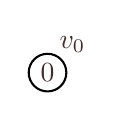
\begin{tikzpicture}[x=0.5pt,y=0.5pt,yscale=-1,xscale=1]
        %uncomment if require: \path (0,306); %set diagram left start at 0, and has height of 306


        % Text Node
        \draw  [line width=0.75]   (92, 109) circle [x radius= 13.6, y radius= 13.6]   ;
        \draw (92,109) node [color={rgb, 255:red, 62; green, 45; blue, 45 }  ,opacity=1 ]  {$0$};
        % Text Node
        \draw (110,89) node [color={rgb, 255:red, 62; green, 45; blue, 45 }  ,opacity=1 ]  {$v_{0}$};


        \end{tikzpicture}

        \\

        \item Видим входной символ '$a$', ищем соответствующую ему операцию в управляющей таблице~--- $shift\ 2$, строим новый узел $v_1$: \\ \\
        Вход: \,
        \begin{tabular}[c]{ |c|c|c|c| }
            \hline \textcolor{red}{a} & b & c & \$ \\ \hline
        \end{tabular}
        \qquad GSS: \,
                \begin{tikzpicture}[x=0.5pt,y=0.5pt,yscale=-1,xscale=1]
        %uncomment if require: \path (0,306); %set diagram left start at 0, and has height of 306


        % Text Node
        \draw  [line width=0.75]   (92, 109) circle [x radius= 13.6, y radius= 13.6]   ;
        \draw (92,109) node [color={rgb, 255:red, 62; green, 45; blue, 45 }  ,opacity=1 ]  {$0$};
        % Text Node
        \draw  [line width=0.75]   (138,98) -- (156,98) -- (156,122) -- (138,122) -- cycle  ;
        \draw (147,110) node [scale=1,color={rgb, 255:red, 62; green, 45; blue, 45 }  ,opacity=1 ]  {а};
        % Text Node
        \draw  [line width=0.75]   (203, 110) circle [x radius= 13.6, y radius= 13.6]   ;
        \draw (203,110) node [color={rgb, 255:red, 62; green, 45; blue, 45 }  ,opacity=1 ]  {$2$};
        % Text Node
        \draw (110,89) node [color={rgb, 255:red, 62; green, 45; blue, 45 }  ,opacity=1 ]  {$v_{0}$};
        % Text Node
        \draw (220,89) node [color={rgb, 255:red, 62; green, 45; blue, 45 }  ,opacity=1 ]  {$v_{1}$};
        % Connection
        \draw    (138,109.84) -- (107.6,109.28) ;
        \draw [shift={(105.6,109.25)}, rotate = 361.03999999999996] [color={rgb, 255:red, 0; green, 0; blue, 0 }  ][line width=0.75]    (10.93,-3.29) .. controls (6.95,-1.4) and (3.31,-0.3) .. (0,0) .. controls (3.31,0.3) and (6.95,1.4) .. (10.93,3.29)   ;

        % Connection
        \draw    (189.4,110) -- (158,110) ;
        \draw [shift={(156,110)}, rotate = 360] [color={rgb, 255:red, 0; green, 0; blue, 0 }  ][line width=0.75]    (10.93,-3.29) .. controls (6.95,-1.4) and (3.31,-0.3) .. (0,0) .. controls (3.31,0.3) and (6.95,1.4) .. (10.93,3.29)   ;


        \end{tikzpicture}

        \\

        \item Повторяем для символа '$b$', операции $shift\ 3$ и узла $v_2$: \\ \\
        Вход: \,
        \begin{tabular}[c]{ |c|c|c|c| }
            \hline a & \textcolor{red}{b} & c & \$ \\ \hline
        \end{tabular}
        \qquad GSS: \,
                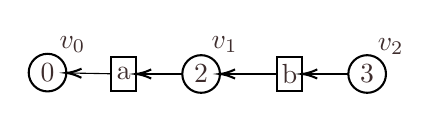
\begin{tikzpicture}[x=0.5pt,y=0.5pt,yscale=-1,xscale=1]
        %uncomment if require: \path (0,306); %set diagram left start at 0, and has height of 306


        % Text Node
        \draw  [line width=0.75]   (92, 109) circle [x radius= 13.6, y radius= 13.6]   ;
        \draw (92,109) node [color={rgb, 255:red, 62; green, 45; blue, 45 }  ,opacity=1 ]  {$0$};
        % Text Node
        \draw  [line width=0.75]   (138,98) -- (156,98) -- (156,122) -- (138,122) -- cycle  ;
        \draw (147,110) node [scale=1,color={rgb, 255:red, 62; green, 45; blue, 45 }  ,opacity=1 ]  {a};
        % Text Node
        \draw  [line width=0.75]   (203, 110) circle [x radius= 13.6, y radius= 13.6]   ;
        \draw (203,110) node [color={rgb, 255:red, 62; green, 45; blue, 45 }  ,opacity=1 ]  {$2$};
        % Text Node
        \draw (110,89) node [color={rgb, 255:red, 62; green, 45; blue, 45 }  ,opacity=1 ]  {$v_{0}$};
        % Text Node
        \draw (220,89) node [color={rgb, 255:red, 62; green, 45; blue, 45 }  ,opacity=1 ]  {$v_{1}$};
        % Text Node
        \draw  [line width=0.75]   (258,98) -- (276,98) -- (276,122) -- (258,122) -- cycle  ;
        \draw (267,110) node [scale=1,color={rgb, 255:red, 62; green, 45; blue, 45 }  ,opacity=1 ]  {b};
        % Text Node
        \draw  [line width=0.75]   (323, 110) circle [x radius= 13.6, y radius= 13.6]   ;
        \draw (323,110) node [color={rgb, 255:red, 62; green, 45; blue, 45 }  ,opacity=1 ]  {$3$};
        % Text Node
        \draw (340,90) node [color={rgb, 255:red, 62; green, 45; blue, 45 }  ,opacity=1 ]  {$v_{2}$};
        % Connection
        \draw    (138,109.84) -- (107.6,109.28) ;
        \draw [shift={(105.6,109.25)}, rotate = 361.03999999999996] [color={rgb, 255:red, 0; green, 0; blue, 0 }  ][line width=0.75]    (10.93,-3.29) .. controls (6.95,-1.4) and (3.31,-0.3) .. (0,0) .. controls (3.31,0.3) and (6.95,1.4) .. (10.93,3.29)   ;

        % Connection
        \draw    (189.4,110) -- (158,110) ;
        \draw [shift={(156,110)}, rotate = 360] [color={rgb, 255:red, 0; green, 0; blue, 0 }  ][line width=0.75]    (10.93,-3.29) .. controls (6.95,-1.4) and (3.31,-0.3) .. (0,0) .. controls (3.31,0.3) and (6.95,1.4) .. (10.93,3.29)   ;

        % Connection
        \draw    (309.4,110) -- (278,110) ;
        \draw [shift={(276,110)}, rotate = 360] [color={rgb, 255:red, 0; green, 0; blue, 0 }  ][line width=0.75]    (10.93,-3.29) .. controls (6.95,-1.4) and (3.31,-0.3) .. (0,0) .. controls (3.31,0.3) and (6.95,1.4) .. (10.93,3.29)   ;

        % Connection
        \draw    (258,110) -- (218.6,110) ;
        \draw [shift={(216.6,110)}, rotate = 360] [color={rgb, 255:red, 0; green, 0; blue, 0 }  ][line width=0.75]    (10.93,-3.29) .. controls (6.95,-1.4) and (3.31,-0.3) .. (0,0) .. controls (3.31,0.3) and (6.95,1.4) .. (10.93,3.29)   ;


        \end{tikzpicture}

        \\

        \item При обработке узла $v_3$ у нас возникает конфликт shift-reduce: $s_6,\ r_3$. Мы смотрим на вершины, смежные $v_2$, на управляющую таблицу и на правило вывода под номером 3 для поиска альтернативного построения стека. Находим $goto\ 4$ и строим вершину $v_3$ с соответствующим переходом по нетерминалу $B$ из $v_1$ (т.к. количество символов в правой части правила вывода 3 равняется 1, значит мы в дереве опустимся на глубину 1 по вершинам-состояниям):\\ \\
        Вход: \,
        \begin{tabular}[c]{ |c|c|c|c| }
            \hline a & b & c & \$ \\ \hline
        \end{tabular}
        \qquad GSS: \,
        \input{part_02_Foundations/chapter_07_ClassicalParsing/figures/05_BottomUp/05_BottomUp_fig_04.tex}
        \\

        \item Читаем символ '$c$' и ищем в управляющей таблице переходы из состояний 3 и 4 (так как узлы $v_2$ и $v_3$ находятся на одном уровне, то есть были построены после чтения одного символа из входного слова). Таким переходом оказывается $s_6$ в обоих случаях, поэтому соединяем узел $v_4$ с обоими рассмотренными узлами:\\ \\
        Вход: \,
        \begin{tabular}[c]{ |c|c|c|c| }
            \hline a & b & \textcolor{red}{c} & \$ \\ \hline
        \end{tabular}
        \qquad GSS: \,
                \begin{tikzpicture}[x=0.5pt,y=0.5pt,yscale=-1,xscale=1]
        %uncomment if require: \path (0,422); %set diagram left start at 0, and has height of 422


        % Text Node
        \draw  [line width=0.75]   (92, 110) circle [x radius= 13.6, y radius= 13.6]   ;
        \draw (92,110) node [color={rgb, 255:red, 62; green, 45; blue, 45 }  ,opacity=1 ]  {$0$};
        % Text Node
        \draw  [line width=0.75]   (138,98) -- (156,98) -- (156,122) -- (138,122) -- cycle  ;
        \draw (147,110) node [scale=1,color={rgb, 255:red, 62; green, 45; blue, 45 }  ,opacity=1 ]  {а};
        % Text Node
        \draw  [line width=0.75]   (203, 110) circle [x radius= 13.6, y radius= 13.6]   ;
        \draw (203,110) node [color={rgb, 255:red, 62; green, 45; blue, 45 }  ,opacity=1 ]  {$2$};
        % Text Node
        \draw (110,89) node [color={rgb, 255:red, 62; green, 45; blue, 45 }  ,opacity=1 ]  {$v_{0}$};
        % Text Node
        \draw (220,89) node [color={rgb, 255:red, 62; green, 45; blue, 45 }  ,opacity=1 ]  {$v_{1}$};
        % Text Node
        \draw  [line width=0.75]   (258,98) -- (276,98) -- (276,122) -- (258,122) -- cycle  ;
        \draw (267,110) node [scale=1,color={rgb, 255:red, 62; green, 45; blue, 45 }  ,opacity=1 ]  {b};
        % Text Node
        \draw  [line width=0.75]   (323, 110) circle [x radius= 13.6, y radius= 13.6]   ;
        \draw (323,110) node [color={rgb, 255:red, 62; green, 45; blue, 45 }  ,opacity=1 ]  {$3$};
        % Text Node
        \draw (340,90) node [color={rgb, 255:red, 62; green, 45; blue, 45 }  ,opacity=1 ]  {$v_{2}$};
        % Text Node
        \draw  [line width=0.75]   (258,158) -- (276,158) -- (276,182) -- (258,182) -- cycle  ;
        \draw (267,170) node [scale=1,color={rgb, 255:red, 62; green, 45; blue, 45 }  ,opacity=1 ]  {B};
        % Text Node
        \draw  [line width=0.75]   (323, 170) circle [x radius= 13.6, y radius= 13.6]   ;
        \draw (323,170) node [color={rgb, 255:red, 62; green, 45; blue, 45 }  ,opacity=1 ]  {$4$};
        % Text Node
        \draw (340,149) node [color={rgb, 255:red, 62; green, 45; blue, 45 }  ,opacity=1 ]  {$v_{3}$};
        % Text Node
        \draw  [line width=0.75]   (374,98) -- (392,98) -- (392,122) -- (374,122) -- cycle  ;
        \draw (383,110) node [scale=1,color={rgb, 255:red, 62; green, 45; blue, 45 }  ,opacity=1 ]  {c};
        % Text Node
        \draw  [line width=0.75]   (374,158) -- (392,158) -- (392,182) -- (374,182) -- cycle  ;
        \draw (383,170) node [scale=1,color={rgb, 255:red, 62; green, 45; blue, 45 }  ,opacity=1 ]  {c};
        % Text Node
        \draw  [line width=0.75]   (437, 110) circle [x radius= 13.6, y radius= 13.6]   ;
        \draw (437,110) node [color={rgb, 255:red, 62; green, 45; blue, 45 }  ,opacity=1 ]  {$6$};
        % Text Node
        \draw (450,89) node [color={rgb, 255:red, 62; green, 45; blue, 45 }  ,opacity=1 ]  {$v_{4}$};
        % Connection
        \draw    (138,110) -- (107.6,110) ;
        \draw [shift={(105.6,110)}, rotate = 360] [color={rgb, 255:red, 0; green, 0; blue, 0 }  ][line width=0.75]    (10.93,-3.29) .. controls (6.95,-1.4) and (3.31,-0.3) .. (0,0) .. controls (3.31,0.3) and (6.95,1.4) .. (10.93,3.29)   ;

        % Connection
        \draw    (189.4,110) -- (158,110) ;
        \draw [shift={(156,110)}, rotate = 360] [color={rgb, 255:red, 0; green, 0; blue, 0 }  ][line width=0.75]    (10.93,-3.29) .. controls (6.95,-1.4) and (3.31,-0.3) .. (0,0) .. controls (3.31,0.3) and (6.95,1.4) .. (10.93,3.29)   ;

        % Connection
        \draw    (309.4,110) -- (278,110) ;
        \draw [shift={(276,110)}, rotate = 360] [color={rgb, 255:red, 0; green, 0; blue, 0 }  ][line width=0.75]    (10.93,-3.29) .. controls (6.95,-1.4) and (3.31,-0.3) .. (0,0) .. controls (3.31,0.3) and (6.95,1.4) .. (10.93,3.29)   ;

        % Connection
        \draw    (258,110) -- (218.6,110) ;
        \draw [shift={(216.6,110)}, rotate = 360] [color={rgb, 255:red, 0; green, 0; blue, 0 }  ][line width=0.75]    (10.93,-3.29) .. controls (6.95,-1.4) and (3.31,-0.3) .. (0,0) .. controls (3.31,0.3) and (6.95,1.4) .. (10.93,3.29)   ;

        % Connection
        \draw    (309.4,170) -- (278,170) ;
        \draw [shift={(276,170)}, rotate = 360] [color={rgb, 255:red, 0; green, 0; blue, 0 }  ][line width=0.75]    (10.93,-3.29) .. controls (6.95,-1.4) and (3.31,-0.3) .. (0,0) .. controls (3.31,0.3) and (6.95,1.4) .. (10.93,3.29)   ;

        % Connection
        \draw    (258,168.07) .. controls (230.15,163.58) and (213.3,149.18) .. (207.42,124.89) ;
        \draw [shift={(206.99,123.01)}, rotate = 437.91] [color={rgb, 255:red, 0; green, 0; blue, 0 }  ][line width=0.75]    (10.93,-3.29) .. controls (6.95,-1.4) and (3.31,-0.3) .. (0,0) .. controls (3.31,0.3) and (6.95,1.4) .. (10.93,3.29)   ;

        % Connection
        \draw    (374,110) -- (338.6,110) ;
        \draw [shift={(336.6,110)}, rotate = 360] [color={rgb, 255:red, 0; green, 0; blue, 0 }  ][line width=0.75]    (10.93,-3.29) .. controls (6.95,-1.4) and (3.31,-0.3) .. (0,0) .. controls (3.31,0.3) and (6.95,1.4) .. (10.93,3.29)   ;

        % Connection
        \draw    (423.4,110) -- (394,110) ;
        \draw [shift={(392,110)}, rotate = 360] [color={rgb, 255:red, 0; green, 0; blue, 0 }  ][line width=0.75]    (10.93,-3.29) .. controls (6.95,-1.4) and (3.31,-0.3) .. (0,0) .. controls (3.31,0.3) and (6.95,1.4) .. (10.93,3.29)   ;

        % Connection
        \draw    (435.82,123.55) .. controls (435.9,150.31) and (416.89,165.24) .. (393.78,168.34) ;
        \draw [shift={(392,168.55)}, rotate = 353.9] [color={rgb, 255:red, 0; green, 0; blue, 0 }  ][line width=0.75]    (10.93,-3.29) .. controls (6.95,-1.4) and (3.31,-0.3) .. (0,0) .. controls (3.31,0.3) and (6.95,1.4) .. (10.93,3.29)   ;

        % Connection
        \draw    (374,170) -- (338.6,170) ;
        \draw [shift={(336.6,170)}, rotate = 360] [color={rgb, 255:red, 0; green, 0; blue, 0 }  ][line width=0.75]    (10.93,-3.29) .. controls (6.95,-1.4) and (3.31,-0.3) .. (0,0) .. controls (3.31,0.3) and (6.95,1.4) .. (10.93,3.29)   ;


        \end{tikzpicture}

        \\

        \item При обработке узла $v_4$ находим соответствующую 6-ому состоянию редукцию по правилу 4. Его правая часть содержит один символ '$c$', 2 вершины-символа с которым достижимы из $v_4$. Находим вершины-состояния, которые смежны с этими вершинами-символами и обрабатываем переходы по левой части правила 4. Такими переходами по нетерминалу $C$ оказываются $5$ и $7$. Строим соответствующие им вершины $v_5$ и $v_6$:\\ \\
        Вход: \,
        \begin{tabular}[c]{ |c|c|c|c| }
            \hline a & b & c & \$ \\ \hline
        \end{tabular}
        \qquad GSS: \,
        \input{part_02_Foundations/chapter_07_ClassicalParsing/figures/05_BottomUp/05_BottomUp_fig_06.tex}
        \\

        \item При обработке узлов $v_5$ и $v_6$ находим редукции с символом '$S$' в левой части и тремя символами в правой. Возвращаемся на 3 вершины-состояния назад и строим вершину $v_7$ с переходом по $S$: \\ \\
        Вход: \,
        \begin{tabular}[c]{ |c|c|c|c| }
            \hline a & b & c & \$ \\ \hline
        \end{tabular}
        \qquad GSS: \,
                \begin{tikzpicture}[x=0.5pt,y=0.5pt,yscale=-1,xscale=1]
        %uncomment if require: \path (0,422); %set diagram left start at 0, and has height of 422


        % Text Node
        \draw  [line width=0.75]   (92, 110) circle [x radius= 13.6, y radius= 13.6]   ;
        \draw (92,110) node [color={rgb, 255:red, 62; green, 45; blue, 45 }  ,opacity=1 ]  {$0$};
        % Text Node
        \draw  [line width=0.75]   (138,98) -- (156,98) -- (156,122) -- (138,122) -- cycle  ;
        \draw (147,110) node [scale=1,color={rgb, 255:red, 62; green, 45; blue, 45 }  ,opacity=1 ]  {а};
        % Text Node
        \draw  [line width=0.75]   (203, 110) circle [x radius= 13.6, y radius= 13.6]   ;
        \draw (203,110) node [color={rgb, 255:red, 62; green, 45; blue, 45 }  ,opacity=1 ]  {$2$};
        % Text Node
        \draw (110,89) node [color={rgb, 255:red, 62; green, 45; blue, 45 }  ,opacity=1 ]  {$v_{0}$};
        % Text Node
        \draw (220,89) node [color={rgb, 255:red, 62; green, 45; blue, 45 }  ,opacity=1 ]  {$v_{1}$};
        % Text Node
        \draw  [line width=0.75]   (258,98) -- (276,98) -- (276,122) -- (258,122) -- cycle  ;
        \draw (267,110) node [scale=1,color={rgb, 255:red, 62; green, 45; blue, 45 }  ,opacity=1 ]  {b};
        % Text Node
        \draw  [line width=0.75]   (323, 110) circle [x radius= 13.6, y radius= 13.6]   ;
        \draw (323,110) node [color={rgb, 255:red, 62; green, 45; blue, 45 }  ,opacity=1 ]  {$3$};
        % Text Node
        \draw (340,90) node [color={rgb, 255:red, 62; green, 45; blue, 45 }  ,opacity=1 ]  {$v_{2}$};
        % Text Node
        \draw  [line width=0.75]   (258,158) -- (276,158) -- (276,182) -- (258,182) -- cycle  ;
        \draw (267,170) node [scale=1,color={rgb, 255:red, 62; green, 45; blue, 45 }  ,opacity=1 ]  {B};
        % Text Node
        \draw  [line width=0.75]   (323, 170) circle [x radius= 13.6, y radius= 13.6]   ;
        \draw (323,170) node [color={rgb, 255:red, 62; green, 45; blue, 45 }  ,opacity=1 ]  {$4$};
        % Text Node
        \draw (340,149) node [color={rgb, 255:red, 62; green, 45; blue, 45 }  ,opacity=1 ]  {$v_{3}$};
        % Text Node
        \draw  [line width=0.75]   (374,98) -- (392,98) -- (392,122) -- (374,122) -- cycle  ;
        \draw (383,110) node [scale=1,color={rgb, 255:red, 62; green, 45; blue, 45 }  ,opacity=1 ]  {c};
        % Text Node
        \draw  [line width=0.75]   (374,158) -- (392,158) -- (392,182) -- (374,182) -- cycle  ;
        \draw (383,170) node [scale=1,color={rgb, 255:red, 62; green, 45; blue, 45 }  ,opacity=1 ]  {c};
        % Text Node
        \draw  [line width=0.75]   (437, 110) circle [x radius= 13.6, y radius= 13.6]   ;
        \draw (437,110) node [color={rgb, 255:red, 62; green, 45; blue, 45 }  ,opacity=1 ]  {$6$};
        % Text Node
        \draw (450,89) node [color={rgb, 255:red, 62; green, 45; blue, 45 }  ,opacity=1 ]  {$v_{4}$};
        % Text Node
        \draw  [line width=0.75]   (372,38) -- (392,38) -- (392,62) -- (372,62) -- cycle  ;
        \draw (382,50) node [scale=1,color={rgb, 255:red, 62; green, 45; blue, 45 }  ,opacity=1 ]  {C};
        % Text Node
        \draw  [line width=0.75]   (372,218) -- (392,218) -- (392,242) -- (372,242) -- cycle  ;
        \draw (382,230) node [scale=1,color={rgb, 255:red, 62; green, 45; blue, 45 }  ,opacity=1 ]  {C};
        % Text Node
        \draw  [line width=0.75]   (437, 50) circle [x radius= 13.6, y radius= 13.6]   ;
        \draw (437,50) node [color={rgb, 255:red, 62; green, 45; blue, 45 }  ,opacity=1 ]  {$5$};
        % Text Node
        \draw  [line width=0.75]   (437, 231) circle [x radius= 13.6, y radius= 13.6]   ;
        \draw (437,231) node [color={rgb, 255:red, 62; green, 45; blue, 45 }  ,opacity=1 ]  {$7$};
        % Text Node
        \draw (452,28) node [color={rgb, 255:red, 62; green, 45; blue, 45 }  ,opacity=1 ]  {$v_{5}$};
        % Text Node
        \draw (452,208) node [color={rgb, 255:red, 62; green, 45; blue, 45 }  ,opacity=1 ]  {$v_{6}$};
        % Text Node
        \draw  [line width=0.75]   (373,278) -- (391,278) -- (391,302) -- (373,302) -- cycle  ;
        \draw (382,290) node [scale=1,color={rgb, 255:red, 62; green, 45; blue, 45 }  ,opacity=1 ]  {S};
        % Text Node
        \draw  [line width=0.75]   (437, 290) circle [x radius= 13.6, y radius= 13.6]   ;
        \draw (437,290) node [color={rgb, 255:red, 62; green, 45; blue, 45 }  ,opacity=1 ]  {$1$};
        % Text Node
        \draw (452,268) node [color={rgb, 255:red, 62; green, 45; blue, 45 }  ,opacity=1 ]  {$v_{7}$};
        % Connection
        \draw    (138,110) -- (107.6,110) ;
        \draw [shift={(105.6,110)}, rotate = 360] [color={rgb, 255:red, 0; green, 0; blue, 0 }  ][line width=0.75]    (10.93,-3.29) .. controls (6.95,-1.4) and (3.31,-0.3) .. (0,0) .. controls (3.31,0.3) and (6.95,1.4) .. (10.93,3.29)   ;

        % Connection
        \draw    (189.4,110) -- (158,110) ;
        \draw [shift={(156,110)}, rotate = 360] [color={rgb, 255:red, 0; green, 0; blue, 0 }  ][line width=0.75]    (10.93,-3.29) .. controls (6.95,-1.4) and (3.31,-0.3) .. (0,0) .. controls (3.31,0.3) and (6.95,1.4) .. (10.93,3.29)   ;

        % Connection
        \draw    (309.4,110) -- (278,110) ;
        \draw [shift={(276,110)}, rotate = 360] [color={rgb, 255:red, 0; green, 0; blue, 0 }  ][line width=0.75]    (10.93,-3.29) .. controls (6.95,-1.4) and (3.31,-0.3) .. (0,0) .. controls (3.31,0.3) and (6.95,1.4) .. (10.93,3.29)   ;

        % Connection
        \draw    (258,110) -- (218.6,110) ;
        \draw [shift={(216.6,110)}, rotate = 360] [color={rgb, 255:red, 0; green, 0; blue, 0 }  ][line width=0.75]    (10.93,-3.29) .. controls (6.95,-1.4) and (3.31,-0.3) .. (0,0) .. controls (3.31,0.3) and (6.95,1.4) .. (10.93,3.29)   ;

        % Connection
        \draw    (309.4,170) -- (278,170) ;
        \draw [shift={(276,170)}, rotate = 360] [color={rgb, 255:red, 0; green, 0; blue, 0 }  ][line width=0.75]    (10.93,-3.29) .. controls (6.95,-1.4) and (3.31,-0.3) .. (0,0) .. controls (3.31,0.3) and (6.95,1.4) .. (10.93,3.29)   ;

        % Connection
        \draw    (258,168.07) .. controls (230.15,163.58) and (213.3,149.18) .. (207.42,124.89) ;
        \draw [shift={(206.99,123.01)}, rotate = 437.91] [color={rgb, 255:red, 0; green, 0; blue, 0 }  ][line width=0.75]    (10.93,-3.29) .. controls (6.95,-1.4) and (3.31,-0.3) .. (0,0) .. controls (3.31,0.3) and (6.95,1.4) .. (10.93,3.29)   ;

        % Connection
        \draw    (374,110) -- (338.6,110) ;
        \draw [shift={(336.6,110)}, rotate = 360] [color={rgb, 255:red, 0; green, 0; blue, 0 }  ][line width=0.75]    (10.93,-3.29) .. controls (6.95,-1.4) and (3.31,-0.3) .. (0,0) .. controls (3.31,0.3) and (6.95,1.4) .. (10.93,3.29)   ;

        % Connection
        \draw    (423.4,110) -- (394,110) ;
        \draw [shift={(392,110)}, rotate = 360] [color={rgb, 255:red, 0; green, 0; blue, 0 }  ][line width=0.75]    (10.93,-3.29) .. controls (6.95,-1.4) and (3.31,-0.3) .. (0,0) .. controls (3.31,0.3) and (6.95,1.4) .. (10.93,3.29)   ;

        % Connection
        \draw    (435.82,123.55) .. controls (435.9,150.31) and (416.89,165.24) .. (393.78,168.34) ;
        \draw [shift={(392,168.55)}, rotate = 353.9] [color={rgb, 255:red, 0; green, 0; blue, 0 }  ][line width=0.75]    (10.93,-3.29) .. controls (6.95,-1.4) and (3.31,-0.3) .. (0,0) .. controls (3.31,0.3) and (6.95,1.4) .. (10.93,3.29)   ;

        % Connection
        \draw    (374,170) -- (338.6,170) ;
        \draw [shift={(336.6,170)}, rotate = 360] [color={rgb, 255:red, 0; green, 0; blue, 0 }  ][line width=0.75]    (10.93,-3.29) .. controls (6.95,-1.4) and (3.31,-0.3) .. (0,0) .. controls (3.31,0.3) and (6.95,1.4) .. (10.93,3.29)   ;

        % Connection
        \draw    (372,50.52) .. controls (341.88,50.18) and (326.06,64.88) .. (324.53,94.64) ;
        \draw [shift={(324.46,96.48)}, rotate = 271.78] [color={rgb, 255:red, 0; green, 0; blue, 0 }  ][line width=0.75]    (10.93,-3.29) .. controls (6.95,-1.4) and (3.31,-0.3) .. (0,0) .. controls (3.31,0.3) and (6.95,1.4) .. (10.93,3.29)   ;

        % Connection
        \draw    (372,229.65) .. controls (341.88,230.53) and (326.05,215.79) .. (324.5,185.41) ;
        \draw [shift={(324.42,183.53)}, rotate = 448.21] [color={rgb, 255:red, 0; green, 0; blue, 0 }  ][line width=0.75]    (10.93,-3.29) .. controls (6.95,-1.4) and (3.31,-0.3) .. (0,0) .. controls (3.31,0.3) and (6.95,1.4) .. (10.93,3.29)   ;

        % Connection
        \draw    (423.4,50) -- (394,50) ;
        \draw [shift={(392,50)}, rotate = 360] [color={rgb, 255:red, 0; green, 0; blue, 0 }  ][line width=0.75]    (10.93,-3.29) .. controls (6.95,-1.4) and (3.31,-0.3) .. (0,0) .. controls (3.31,0.3) and (6.95,1.4) .. (10.93,3.29)   ;

        % Connection
        \draw    (423.4,230.75) -- (394,230.22) ;
        \draw [shift={(392,230.18)}, rotate = 361.03999999999996] [color={rgb, 255:red, 0; green, 0; blue, 0 }  ][line width=0.75]    (10.93,-3.29) .. controls (6.95,-1.4) and (3.31,-0.3) .. (0,0) .. controls (3.31,0.3) and (6.95,1.4) .. (10.93,3.29)   ;

        % Connection
        \draw    (423.4,290) -- (393,290) ;
        \draw [shift={(391,290)}, rotate = 360] [color={rgb, 255:red, 0; green, 0; blue, 0 }  ][line width=0.75]    (10.93,-3.29) .. controls (6.95,-1.4) and (3.31,-0.3) .. (0,0) .. controls (3.31,0.3) and (6.95,1.4) .. (10.93,3.29)   ;

        % Connection
        \draw    (373,289.72) .. controls (234.96,286.59) and (143.34,231.38) .. (98.15,124.08) ;
        \draw [shift={(97.47,122.46)}, rotate = 427.47] [color={rgb, 255:red, 0; green, 0; blue, 0 }  ][line width=0.75]    (10.93,-3.29) .. controls (6.95,-1.4) and (3.31,-0.3) .. (0,0) .. controls (3.31,0.3) and (6.95,1.4) .. (10.93,3.29)   ;


        \end{tikzpicture}

        \\
        \item Наконец, обрабатывая вершину $v_7$, читаем символ '$\$$' и строим узел $v_8$, который соответствует допускающим состоянием: \\ \\
        Вход: \,
        \begin{tabular}[c]{ |c|c|c|c| }
            \hline a & b & c & \textcolor{red}{\$} \\ \hline
        \end{tabular}
        \qquad GSS: \,
        \input{part_02_Foundations/chapter_07_ClassicalParsing/figures/05_BottomUp/05_BottomUp_fig_08.tex}
        \\
    \end{enumerate}



\end{example}

\section{Сравнение классов LL и LR}

Иерархию языков, распознаваемых различными классами алгоритмов, можно представить как изображено на рисунке~\ref{fig:ll_lr_comparison}.

\begin{marginfigure}
\begin{center}
  \input{part_02_Foundations/chapter_07_ClassicalParsing/figures/06_LLvsLR/LL_LR}
\end{center}
\caption{Соотношение между классами $LL(k)$ и $LR(k)$}
\label{fig:ll_lr_comparison}
\end{marginfigure}

Из диаграммы видно, что класс языков, распознаваемых LL(k) алгоритмом уже, чем класс языков, распознаваемый LR(k) алгоритмом, при любом конечном $k$. Приведём несколько примеров.
\begin{enumerate}
\item $L = \{a^mb^nc \mid m \geq n \geq 0\} $ является LR(0), но для него не существует LL(1) грамматики.
\item $L = \{ a^n b^n + a^n c^n \mid n > 0\}$ является LR, но не LL.
\item Больше примеров можно найти в работе Джона Битти~\cite{BEATTY1980193}.
\end{enumerate}

